\documentclass[10pt,letterpaper,journal]{IEEEtran}
\usepackage[T1]{fontenc}
\usepackage{amsmath,amsthm,graphicx,booktabs,array,url}
\usepackage{newtxtext,newtxmath}
\usepackage{microtype}
\usepackage{cite}
\usepackage{balance}
\usepackage[hidelinks]{hyperref}
\usepackage{adjustbox}
\setlength{\textwidth}{7in}
\setlength{\textheight}{9.5in}
\setlength{\oddsidemargin}{-0.25in}
\setlength{\evensidemargin}{-0.25in}
\setlength{\topmargin}{-0.80in}
\setlength{\columnsep}{0.30in}
\setlength{\parindent}{12pt}
\setlength{\parskip}{3pt}
\makeatletter
\def\ps@headings{\let\@oddhead\@empty\let\@evenhead\@empty%
\def\@oddfoot{\hfil\normalfont\fontsize{9}{10}\selectfont\thepage\hfil}%
\let\@evenfoot\@oddfoot}
\let\ps@IEEEtitlepagestyle\ps@headings
\makeatother
\pagestyle{headings}
\newtheorem{theorem}{Theorem}
\newtheorem{proposition}{Proposition}
\newtheorem{lemma}{Lemma}
\newtheorem{remark}{Remark}
\newtheorem{corollary}{Corollary}
\newcommand{\R}{\mathbb{R}}
% Auto-generated; do not edit by hand.
\newcommand{\CTwoWins}{11}
\newcommand{\CTwoLosses}{8}
\newcommand{\CTwoCases}{20}
\newcommand{\CTwoRank}{0.74}
\newcommand{\CTwoMedian}{+4.1}
\newcommand{\CTwoFixedWins}{3}
\newcommand{\CTwoFixedLosses}{9}
\newcommand{\CTwoGateWins}{14}
\newcommand{\CTwoGateLosses}{6}
\newcommand{\CTwoVoneWins}{8}
\newcommand{\CTwoVoneLosses}{12}
\newcommand{\CTwoVoneRank}{0.26}
\newcommand{\CThreeZero}{21}
\newcommand{\CThreeZeroMax}{43}
\newcommand{\CThreeFive}{2.3}
\newcommand{\CThreeIBM}{0.004}
\newcommand{\CFourRobust}{1.000}
\newcommand{\CFourPlugin}{0.502}
\newcommand{\CFourInside}{0}
\newcommand{\CFourInsideCases}{30}
\newcommand{\CFourPlainInside}{0}
\newcommand{\CFourPlainOutside}{6}
\newcommand{\CFourOutsideCases}{12}
\newcommand{\CFourExtendedOutside}{0}
\newcommand{\CFourTrials}{1200}
\newcommand{\CFourSlack}{23}
\newcommand{\CFiveViolations}{3}
\newcommand{\CFiveFalse}{2}
\newcommand{\CFiveCases}{6}
\newcommand{\CSixTrials}{300}
\newcommand{\CSixViolations}{0}
\newcommand{\CEightGates}{133{,}160}
\newcommand{\CEightTime}{1087.7}
\newcommand{\CEightGap}{6e-02}

\title{{\fontsize{17}{20}\selectfont\bfseries Quantum Circuit Optimization Using Geometric Programming:\\ Exact Convex Co-Design of Gate Timing, Dynamical Decoupling, and Error-Mitigation Budgets}}
\author{{\fontsize{11}{13}\selectfont Youssef Ahmed Ramadan}\\[3pt]
{\fontsize{10}{12}\selectfont\itshape Department of Artificial Intelligence Engineering, School of Engineering}\\
{\fontsize{10}{12}\selectfont\itshape University of Science and Technology at Zewail City}\\
{\fontsize{10}{12}\selectfont\itshape Giza, Egypt}\\
{\fontsize{10}{12}\selectfont Email: p-youssef.ramdan@zewailcity.edu.eg}}
\IEEEaftertitletext{%
\vspace{12pt}\par\noindent\hspace*{0.25in}\begin{minipage}{6.5in}
\fontsize{9}{12}\selectfont\noindent\textbf{\textit{Abstract---}} Quantum compilers must decide how long each gate takes, where idle time falls, how idle qubits are dynamically decoupled (DD), and how many shots error mitigation needs. We show that, under Markovian Pauli--Lindblad noise whose rates depend on these resources by power laws, the quantities a compiler cares about---log-fidelity of tracked observables, the sampling overhead of probabilistic error cancellation (PEC), estimator variance, and QPU time---are posynomials or exponentials of posynomials. Their joint allocation is therefore a geometric program (GP), or convex in logarithmic coordinates, and is solved to global optimality with a dual certificate. Gate durations, idle placement and DD pulse counts are jointly convex through a perspective structure, with a closed-form optimal pulse count and a drive-versus-idle threshold; QPU time for PEC-mitigated estimation has the closed-form optimum $\tau_j^\star=\sqrt{a_j/(g_j+p_j/4(M+t_{\rm rep}))}$; an ellipsoidal robust counterpart stays an exact GP with a calibration-coverage certificate, and baseline-dominance constraints guarantee the schedule never loses to a default on any error law in a declared hull; anisotropic, state-aware hazards remain posynomial, while isotropic models provably cannot represent basis-dependent rankings; discrete pulse-library selection is strongly NP-hard, whereas log-grid rounding is a $(q,q)$-bicriteria approximation. In independent time-correlated simulations with models fitted only from spectroscopy, joint timing and DD beats the best of ASAP, ALAP, ALAP+XX and ALAP+XY4 in \CTwoWins{} of \CTwoCases{} cases and loses in \CTwoLosses{}; gains rely on duration control, and low-frequency noise shared across idle windows is the main failure mode. Runtime-optimal PEC saves a median \CThreeZero\% of QPU time without repetition overhead but only \CThreeIBM\% at IBM's default delay, as predicted. Robust certificates cover the true error in all \CFourTrials{} simulated calibrations (frequency \CFourRobust{}) versus \CFourPlugin{} for plug-in predictions, and the earlier 100\% misspecification regression disappears at under 0.3 pp cost. On IBM Heron, in a pre-registered test and replication using about one minute of free-tier QPU time, the model predicted the ranking of five decoupling policies, correctly left a noisy qubit undecoupled, and beat the best standard sequence (XY4) by 2.2 percentage points in all-qubit return probability (pooled 95\% interval 1.4--2.9) on one qubit chain. Pre-registered control arms on that chain and on a second, disjoint chain show that the gain comes from the allocation rather than from pulse count: GP-DD beat a uniform eight-pulse schedule with nearly twice as many pulses by 1.6 points (pooled interval 1.0--2.1). On the second chain, GP-DD tied XY4.\par\vspace{6pt}\noindent\textbf{\textit{Index Terms---}} Quantum compilation, geometric programming, convex optimization, dynamical decoupling, error mitigation, robust optimization, gate scheduling, Heron architecture.\par\end{minipage}\hspace*{0.25in}\par\vspace{12pt}
}
\begin{document}
\maketitle


\section{Introduction}
\IEEEPARstart{Q}{uantum} compilation connects abstract circuits to executable pulses and schedules. Gate count, depth, makespan, and noisy-state fidelity are distinct quantities. Shorter schedules can demand stronger control and may increase error. We therefore study a precise subproblem: duration allocation on a fixed dependency graph under a declared noise model. Its optimum and error bounds are conditional on that model, rather than guarantees about an uncharacterized device.

The mathematical structure of time-cost tradeoffs on directed acyclic dependency graphs (DAGs) traces back to the foundational network-flow duality of Kelley \cite{kelley} and Fulkerson \cite{fulkerson}. Geometric programming (GP) provides an established positive-variable optimization language with an exact convex transformation under logarithmic change of variables \cite{boydgp}. Its historical application to digital CMOS circuit sizing and timing closure played a foundational role in classical electronic design automation (EDA) \cite{boyddigital}. In quantum computing, when gate durations are fixed, makespan minimization reduces to a longest-path computation on a DAG. However, physical quantum devices operate under a different decision space: continuous gate durations and discrete pulse implementations that preserve target local unitaries while trading off drive strength, environmental decoherence, and circuit latency.

The central observation of this paper is that a single mathematical object governs many of these decisions at once. Under Markovian Pauli--Lindblad noise, a stabilizer expectation decays as the exponential of a sum of Pauli intensities, and the PEC overhead is the exponential of their total. If each intensity is a posynomial in the physical resources, every quantity of interest is log-posynomial, and GP supplies global optimality, duality, sensitivity and robust counterparts. Gate-duration allocation on a fixed DAG, studied in Sections~III--VII, is the simplest instance; its convexity and path-flow duality are adaptations of known time--cost results and are presented as preliminaries.

Our contributions are:
\begin{enumerate}
\item a catalogue theorem placing observable constraints, PEC overhead, estimator variance and QPU time in one log-convex class (Theorem~\ref{th:catalogue});
\item joint convexity of gate durations, idle placement and DD pulse counts under power-law dephasing spectra, with a closed-form pulse count, a drive-versus-idle threshold, a state-aware $T_1$ extension and an exact cross-window protection model for fixed schedules (Theorem~\ref{th:dd} and its corollaries);
\item the closed-form runtime-optimal schedule for PEC-mitigated estimation (Theorem~\ref{th:runtime});
\item an exact-GP ellipsoidal robust counterpart with a calibration-coverage guarantee, and baseline dominance on a declared law hull (Theorems~\ref{th:coverage}--\ref{th:dominance});
\item a proof that isotropic noise forces basis-independent rankings, together with anisotropic constraints that remain posynomial (Proposition~\ref{prop:iso});
\item strong NP-hardness of discrete library selection with a $(q,q)$-bicriteria rounding guarantee, and log-log convexity of the latency--fidelity frontier with a dual ``fidelity price'' (Theorems~\ref{th:hard}--\ref{th:bicriteria}, Proposition~\ref{prop:frontier});
\item an independent time-correlated noise simulator, and a pre-registered, replicated hardware test on IBM Heron.
\end{enumerate}
We distinguish model-consistency checks from external validation throughout and report regressions alongside gains.

Sections~II--VII describe prior work, the duration model and its bounds, and the observable formulation. Section~VIII develops the GP resource-allocation framework. Section~IX reports simulations and hardware experiments. Section~X describes the compiler pass and limitations; Section~XI concludes.

\section{Related Work and Scientific Context}
\subsection{Duration-Aware Quantum Scheduling}
Lussi, de Santiago, and Duzzioni recently introduced duration-aware quantum scheduling by assigning fast pulse implementations to critical-path operations and robust, longer implementations to available off-critical slack \cite{lussi}. Our work builds upon this insight by formulating continuous duration allocation as an exact convex program, deriving analytical primal-dual optimality certificates, and incorporating nonunitary open-system channel bounds. In quantum compiler systems, noise-adaptive mapping and crosstalk-aware scheduling have been investigated by Murali et al. \cite{murali_noise,murali_crosstalk}, while pulse-efficient transpilation was developed by Earnest et al. \cite{earnest}. Dynamical decoupling techniques for open quantum systems have been developed to mitigate low-frequency non-Markovian noise during idle intervals \cite{viola_dd,qiskit_sched}.

\subsection{Convex Scheduling and Classical Foundations}
Convex project time-cost optimization on DAGs originates in the classic network-flow duality of Kelley \cite{kelley} and Fulkerson \cite{fulkerson}, subsequently generalized to convex cost dual network flow by Ahuja et al. \cite{ahuja}. Geometric programming supplies an exact convex representation when all cost terms are positive monomials or posynomials \cite{boydgp}. For the proposed inverse-duration-plus-duration costs, the original variables also yield an ordinary convex formulation, establishing that efficiency stems from convexity rather than logarithmic change of variables alone.

\subsection{Noise Modeling and Stabilizer Observables}
The no-jump branch of a quantum-trajectory representation underlies the channel certificate \cite{dalibard}. Conditional-gradient methods provide established optimization-gap machinery \cite{jaggi}. Compositional robustness for quantum programs has been formalized by Hung et al. \cite{hung}, while robust quantum control via sequential convex programming was investigated by Kosut et al. \cite{kosut}. Sparse Pauli-Lindblad noise characterization has been established by van den Berg et al. \cite{vandenberg}. Recently, P.~Aigner et al. \cite{aigner} developed analytical and compressed simulation techniques for noisy stabilizer circuits. Our framework leverages duration-dependent noise sensitivity to convert analytical stabilizer tracking into a posynomial constraint, enabling convex interior-point optimization for compiler scheduling.

\subsection{Decoupling, Error Mitigation, and Discrete Time--Cost Trade-offs}
Filter-function theory relates DD sequences to dephasing spectra \cite{uhrig,cywinski,biercuk}; compiler work selects DD per qubit adaptively \cite{adapt} or variationally \cite{vaqem}, and a survey compares sequences on superconducting hardware \cite{ezzell}. Probabilistic error cancellation is due to Temme et al. \cite{temme} and was scaled with sparse Pauli--Lindblad models \cite{vandenberg}. The discrete time--cost trade-off problem is strongly NP-hard \cite{de1997} and admits bicriteria approximations \cite{skutella}. Recent work learns DD sequences empirically on IBM processors \cite{tong2024} or by closed-loop optimization of rotation angles \cite{rahman2024}, and embeds DD in a context-aware way that suppresses correlated noise and crosstalk \cite{seif2024,coote2024,brown2024}. A 2026 review argues that DD should be treated as a hardware-aware scheduling problem rather than an isolated control protocol \cite{li2026}. On the mitigation side, PEC sampling overhead has recently been reduced by Pauli error propagation \cite{scheiber2025} and by combining error detection with PEC \cite{fischer2026}; our runtime result is complementary, lowering the overhead exponent through scheduling. These methods are heuristic, learned, or graph-based. To our knowledge, no prior work proves joint convexity of gate timing and DD allocation, or derives the runtime-optimal schedule for mitigated estimation.

\section{Preliminaries: Continuous Duration Model and Exact Convexity}
The results of this section and Sections~IV--VII adapt established time--cost and geometric-programming structure \cite{kelley,fulkerson,boydgp,boyddigital} to quantum gate durations. They are the foundation for the new results of Section~\ref{sec:framework}.

Let a native circuit contain $m$ unitary gates and a dependency DAG $\mathcal{D}$ with $r$ edges. Per-qubit order is fixed by the logical circuit; concurrent operations on overlapping qubit supports are forbidden. Gate $i$ has continuous duration $\tau_i \in [\ell_i, u_i]$, with $0 < \ell_i \le u_i$, generated by a Hermitian Hamiltonian $H_i = K_i / \tau_i$ such that
\begin{equation}
e^{-\mathrm{i}K_i} = e^{\mathrm{i}\phi_i}U_i, \quad K_i = \theta_i P_i / 2,
\end{equation}
where $P_i$ denotes the generating Hamiltonian. On superconducting transmon processors such as IBM Heron, native operations comprise single-qubit rotations (SX, X, and virtual RZ) and two-qubit Controlled-Z (CZ) entangling interactions; entangling gates like RXX decompose into native CZ and single-qubit rotations. Because $K_i$ is fixed, the ideal local unitary is duration-independent.

Define the integrated squared control effort $E(\tau) = \sum_i \kappa_i^2 / \tau_i$, where $\kappa_i = \|K_i\|_2$. For a schedule with makespan $M$, the integrated noise hazard satisfies
\begin{equation}\label{eq:risk_model}
\Lambda \le R(\tau, M) = bM + \sum_i \left( \frac{a_i}{\tau_i} + \gamma_i \tau_i \right),
\end{equation}
where $b, a_i, \gamma_i > 0$. The inverse-plus-linear term $a_i/\tau_i + \gamma_i\tau_i$ represents a stylized phenomenological noise model capturing the fundamental engineering tension between drive-power-induced errors (leakage, non-adiabaticity, and amplifier distortion at small $\tau_i$) and environmental decoherence exposure ($T_1, T_2$ relaxation and dephasing at large $\tau_i$).

The objective balances noise hazard, makespan, and control effort:
\begin{equation}\label{eq:objective}
J(\tau, M) = w_R \frac{R}{R_0} + w_M \frac{M}{M_0} + w_E \frac{E}{E_0},
\end{equation}
subject to precedence constraints $f_i + \tau_j \le f_j$ for $(i \to j) \in \mathcal{D}$, completion constraints $\tau_i \le f_i \le M$, and duration bounds $\ell_i \le \tau_i \le u_i$.

\begin{theorem}[Convexity and Conditional Uniqueness]\label{th:exactness}
Suppose $R_0,M_0,E_0>0$, $w_R,w_M,w_E\ge0$, and the gate coefficients are nonnegative. The fixed-DAG duration-allocation problem in \eqref{eq:objective} is an exact geometric program whenever the positive-variable formulation is used, and is convex in the original durations and finish-time variables. Define $A_i=w_Ra_i/R_0+w_E\kappa_i^2/E_0$. If $A_i>0$ for every nonfixed duration coordinate, the optimal duration vector is unique. This does not imply unique intermediate finish times.
\end{theorem}
\begin{proof}
Write $B=w_Rb/R_0+w_M/M_0\ge0$ and $C_i=w_R\gamma_i/R_0\ge0$. Eliminating the finish-time variables at fixed $\tau$ gives the reduced objective
\[F(\tau)=\sum_i(A_i/\tau_i+C_i\tau_i)+B\max_{p\in\mathcal P}p^\top\tau.\]
The box is compact, all reciprocal terms are convex on positive durations, and the maximum of path sums is convex. Hence a minimizer exists. If every free-coordinate $A_i>0$, the Hessian of $\sum_iA_i/\tau_i$ is diagonal with entries $2A_i/\tau_i^3>0$ on the free-coordinate subspace. The reduced objective is then strictly convex, so its minimizing duration vector is unique. For the GP representation, positive monomials and posynomials express the objective and precedence inequalities; logarithmic substitution yields convex log-sum-exp inequalities. Fixed coordinates can be eliminated. A zero coefficient or weight may remove strict convexity, so uniqueness is not asserted outside the stated condition.
\end{proof}

\begin{remark}[Objective Formulation and Non-Uniqueness under Pure Makespan Minimization]\label{rem:uniqueness}
Theorem~\ref{th:exactness} guarantees uniqueness of the optimal duration vector only when the reciprocal error coefficients in the reduced objective function are strictly positive ($w_R > 0$ with $A_i > 0$). In contrast, when the problem is formulated to minimize makespan alone subject to error constraints (as in Algorithm~1), the objective depends exclusively on the critical path length. Gates lying off the critical path possess non-zero slack: their durations can be continuously varied within their slack margins without altering the makespan, provided precedence and observable constraints remain satisfied. Consequently, off-critical duration allocations under pure makespan minimization are non-unique and mathematically arbitrary unless regularized by a strictly convex secondary risk objective.
\end{remark}

\begin{proposition}[Positive Inverse-Power Extension]\label{prop:power}
For a declared exponent $p>0$, replace the reduced duration objective by
\begin{equation}
F_p(\tau)=\sum_i\left(A_i\tau_i^{-p}+C_i\tau_i\right)+B\max_{q\in\mathcal P}q^\top\tau,
\end{equation}
with $A_i,C_i\ge0$, $B>0$, and positive duration bounds. This is a geometric program and is convex in the original durations. If $A_i>0$ for each free coordinate, the optimal duration vector is unique. The path-flow dual of Theorem~\ref{th:dual} remains valid with coordinate response
\begin{equation}
\tau_i(\rho)=\operatorname{clip}\!\left[\left(\frac{pA_i}{C_i+\rho_i}\right)^{1/(p+1)},\ell_i,u_i\right]
\end{equation}
when $C_i+\rho_i>0$; if it is zero and $A_i>0$, the response is $u_i$.
\end{proposition}
\begin{proof}
Each $A_i\tau_i^{-p}$ is a positive monomial, hence the positive-variable objective and precedence ratios satisfy GP grammar. Its second derivative is $p(p+1)A_i\tau_i^{-p-2}\ge0$, strictly positive on free coordinates with $A_i>0$. The maximum of path sums is convex, so strict convexity and uniqueness follow as in Theorem~\ref{th:exactness}. Minimax interchange over the compact duration box and path-flow polytope is unchanged. Differentiating $A_i/t^p+(C_i+\rho_i)t$ gives the displayed clipped minimizer. This extension changes the assumed error law; it does not validate any exponent from hardware data.
\end{proof}

\begin{proposition}[Rectangular Box Robustness]
If each coefficient in \eqref{eq:risk_model} belongs independently to a declared interval $[a_i^{\min}, a_i^{\max}]$, its maximum over that rectangle is attained at the upper endpoints. Replacing coefficients by those endpoints yields an exact robust GP.
\end{proposition}
\begin{proof}
Each coefficient multiplies a nonnegative term, so $R$ is coordinatewise monotone. The upper endpoint vector belongs to the uncertainty rectangle and attains its maximum for every feasible schedule.
\end{proof}

\begin{proposition}[Finite-Scenario Robust GP]\label{prop:scenario}
Let a declared finite set $\mathcal S$ contain nonnegative coefficient pairs $(A_{is},C_{is})$ for a common exponent $p>0$. Under the same positive duration box, DAG constraints, and optional deadline, the minimax problem
\begin{equation}
\min_{\tau,M}\left\{\max_{s\in\mathcal S}\sum_i(A_{is}\tau_i^{-p}+C_{is}\tau_i)+BM\right\}
\end{equation}
is an exact geometric program in epigraph form. Its optimum is robust only with respect to the \emph{declared} scenarios; it is a physical error bound only if the true coefficients are contained in a justified uncertainty set.
\end{proposition}
\begin{proof}
Introduce $z>0$ and require $\sum_i(A_{is}\tau_i^{-p}+C_{is}\tau_i)/z\le1$ for each $s\in\mathcal S$. Every left-hand side is a posynomial, and $z+BM$ is a posynomial objective. The timing and deadline constraints retain GP form. For fixed feasible $\tau$, the smallest feasible $z$ is exactly the maximum scenario error, proving epigraph equivalence. Taking a maximum over finitely many convex scenario errors also proves convexity in the original durations. Nothing in this argument assigns statistical coverage to $\mathcal S$.
\end{proof}

\begin{proposition}[Quantization Rounding Certificate]
If a rounded vector $\tau'$ remains within $[\ell, u]$, then
\begin{equation}
|R(\tau') - R(\tau)| \le \sum_i \left( \frac{a_i}{\ell_i^2} + \gamma_i + b \right) |\tau'_i - \tau_i|.
\end{equation}
\end{proposition}
\begin{proof}
Every path sum changes by at most $\sum_i |\tau'_i - \tau_i|$, bounding makespan change. The derivative magnitude of $a_i/\tau_i + \gamma_i\tau_i$ on $[\ell_i, u_i]$ is bounded by $a_i/\ell_i^2 + \gamma_i$. Summing yields the result.
\end{proof}

\section{Path-Flow Dual and Algorithm}
Let $\mathcal{P}$ denote the set of all root-to-sink path incidence vectors in $\mathcal{D}$. Makespan is $M(\tau) = \max_{p \in \mathcal{P}} p^\top \tau$. Combining objective coefficients into $A_i, C_i > 0$ and $B > 0$, the unconstrained deadline problem becomes
\begin{equation}
\min_{\ell \le \tau \le u} \sum_i \left( \frac{A_i}{\tau_i} + C_i \tau_i \right) + B \max_{p \in \mathcal{P}} p^\top \tau.
\end{equation}

\begin{theorem}[Path-Flow Dual Bracket]\label{th:dual}
For any dual flow vector $\rho \in B \operatorname{conv}(\mathcal{P})$, define the dual objective and duration response:
\begin{align}
D(\rho) &= \sum_i \min_{\ell_i \le t \le u_i} \left[ \frac{A_i}{t} + (C_i + \rho_i)t \right],\\
\tau_i(\rho) &= \operatorname{clip}\left( \sqrt{\frac{A_i}{C_i + \rho_i}}, \ell_i, u_i \right).
\end{align}
Then strong duality holds: $\max_\rho D(\rho) = \min_\tau J(\tau)$. Moreover, every dual-feasible $\rho$ provides an inspectable optimality gap:
\begin{equation}
0 \le J(\tau(\rho)) - J^* \le B M(\tau(\rho)) - \rho^\top \tau(\rho).
\end{equation}
\end{theorem}
\begin{proof}
The set $\mathcal P$ contains every source-to-sink path incidence vector of the fixed DAG; $B\operatorname{conv}(\mathcal P)$ consists exactly of nonnegative path mixtures whose total path weight is $B$. It is compact and convex. For $L(\tau,\rho)=\sum_i(A_i/\tau_i+C_i\tau_i)+\rho^\top\tau$, the duration box is also compact and convex, $L$ is continuous and convex in $\tau$, and it is affine in $\rho$. The minimax theorem interchanges min and max. Since $\max_{\rho\in B\operatorname{conv}(\mathcal P)}\rho^\top\tau=B M(\tau)$, the primal is recovered. Coordinatewise minimization gives $D(\rho)$ and the clipped square-root response. For any feasible $\rho$, weak duality gives $D(\rho)\le J^*$. At $\tau(\rho)$, $J(\tau(\rho))-D(\rho)=B M(\tau(\rho))-\rho^\top\tau(\rho)$. Combining the two inequalities yields the stated upper bound on primal suboptimality.
\end{proof}

Because $\nabla D(\rho) = \tau(\rho)$, a longest-path oracle on the DAG solves the linear subproblem in $\mathcal{O}(m+r)$ time. A conditional gradient (Frank--Wolfe) update $\rho \leftarrow (1-\alpha)\rho + \alpha B p$ with bisection line search guarantees dual-feasible monotonic ascent.

\section{Nonunitary Operational Certificates}
We extend operational guarantees to open quantum systems governed by the Lindblad master equation:
\begin{equation}
\dot\rho = -\mathrm{i}[H(t), \rho] + \sum_\mu \left( L_\mu \rho L_\mu^\dagger - \tfrac{1}{2}\{L_\mu^\dagger L_\mu, \rho\} \right).
\end{equation}
Let $\Delta H(t)$ denote coherent Hamiltonian mismatch, $N = \int \sum_\mu \|L_\mu(t)\|_\infty^2 dt$, and $C = \int \|\Delta H(t)\|_\infty dt$.

For clarity, $F_{\mathrm{pur}}$ below denotes the infimum, over normalized input states with an arbitrary untouched reference, of the squared overlap between the ideal output purification and the implemented output state.
\begin{theorem}[Unitary-jump operational bound]\label{th:noise}
Suppose coherent Hamiltonian mismatch vanishes and $L_\mu(t)=\sqrt{r_\mu(t)}V_\mu(t)$ with $V_\mu^\dagger V_\mu=I$. If $\Lambda=\int\sum_\mu r_\mu(t)\,dt\le R$, then
\begin{align}
F_{\mathrm{pur}}&\ge e^{-R},\\
\tfrac12\|\mathcal N-\mathcal U\|_\diamond&\le1-e^{-R}.
\end{align}
\end{theorem}
\begin{proof}
For every time, $\sum_\mu L_\mu^\dagger L_\mu=h(t)I$ with $h(t)=\sum_\mu r_\mu(t)$. The no-jump propagator is therefore $K_0=e^{-\Lambda/2}U$, even when the unitary jumps do not commute with the control. The trajectory expansion is a sum of completely positive branches, and its no-jump branch is $e^{-\Lambda}\mathcal U$. As the complete map is trace preserving, the sum of all remaining branches is a completely positive map whose output trace is $(1-e^{-\Lambda})\operatorname{Tr}\rho$. After normalization it is a channel $\mathcal Q$ (the $\Lambda=0$ case is immediate). Thus $\mathcal N=e^{-\Lambda}\mathcal U+(1-e^{-\Lambda})\mathcal Q$. Tensoring with any reference preserves the decomposition. The output overlap with the ideal pure state is at least the weight of its ideal branch, proving $F_{\mathrm{pur}}\ge e^{-\Lambda}\ge e^{-R}$. Finally, $\|\mathcal Q-\mathcal U\|_\diamond\le2$ implies the distance bound.
\end{proof}

\begin{proposition}[General Markovian Operational Certificates]\label{prop:nonunitary}
For general Markovian dynamics including non-unital amplitude damping ($T_1$ relaxation via $L = \sigma^-$, where $(\sigma^-)^\dagger \sigma^- \ne I$), with integrable bounds $N$ and $C$, the implemented channel $\mathcal{N}$ and ideal channel $\mathcal{U}$ satisfy:
\begin{align}
\tfrac{1}{2}\|\mathcal{N} - \mathcal{U}\|_\diamond &\le \min(1, N + C),\\
F_{\mathrm{pur}} &\ge \max\left\{ (1 - N - C)_+, \left(1 - \tfrac{N}{2} - C\right)_+^2 \right\}.
\end{align}
\end{proposition}
\begin{proof}
Let $\Gamma(t)=\sum_\mu L_\mu(t)^\dagger L_\mu(t)$ and move to the ideal interaction picture, including an arbitrary untouched reference. The dissipator superoperator has diamond norm at most $2\sum_\mu\|L_\mu(t)\|_\infty^2$; the coherent commutator has diamond norm at most $2\|\Delta H(t)\|_\infty$. Duhamel's formula between CPTP propagators therefore gives $\|\mathcal N-\mathcal U\|_\diamond/2\le N+C$, capped by one. For the second bound, the no-jump interaction-picture operator $K_0$ obeys $\dot K_0=(-i\widetilde{\Delta H}-\widetilde\Gamma/2)K_0$. Its propagator is contractive, and integration gives $\|K_0-I\|_\infty\le C+N/2$. On any normalized input purification $|\psi\rangle$, $|\langle\psi|K_0\otimes I|\psi\rangle|\ge(1-C-N/2)_+$. The no-jump contribution to the output overlap is the square of this amplitude, while all other Kraus contributions are nonnegative. The trace-distance bound independently yields an overlap of at least $(1-N-C)_+$ for a pure ideal output. Taking the better floor and the infimum over inputs proves the claim.
\end{proof}

Our physical spin model uses $K_i = \theta_i P_i/2$. Always-on memory jumps are $\sqrt{1/T_{1q}}\sigma^-_q$ and $\sqrt{1/(2T_{\phi q})}Z_q$, while gate-dependent drive jumps are $\sqrt{\eta_i}K_i/\tau_i$ and $\sqrt{\gamma_i}P_i$. While Theorem~\ref{th:noise} provides an exponential floor for unital jump generators, Proposition~\ref{prop:nonunitary} rigorously bounds general non-unital $T_1$ relaxation.

\section{Discrete Pulse Libraries and Certificate Transfer}
When hardware restricts controls to a discrete pulse library $\{d_{ik}\}_{k=1}^K \subset [\ell_i, u_i]$, duration selection is governed by binary indicators $x_{ik} \in \{0, 1\}$ with $\sum_k x_{ik} = 1$ and $\tau_i = \sum_k d_{ik} x_{ik}$.

For each pulse implementation $\mathcal{E}_{ik}$ and target $\mathcal{U}_i$, let $J_{ik}$ be the unnormalized Choi matrix of their difference. Watrous's SDP \cite{watrous} yields the dual upper bound $\delta_{ik} = \min\{ 1, \tfrac{1}{2}\|\operatorname{Tr}_{\mathrm{out}} |J_{ik}| \|_\infty\}$. Summing over disjoint gates with memory dissipation rate $b_i$ gives compositional channel error $Q(x, M) = bM + \sum_{ik} (\delta_{ik} - b_i d_{ik})x_{ik}$.

\begin{proposition}[GP-to-Library Transfer Bound]\label{prop:transfer}
Let $D_{\mathrm{GP}}$ be a continuous GP dual lower bound. Define residual errors $e_{ik} = (\delta_{ik} - b_i d_{ik} - a_i/d_{ik} - \gamma_i d_{ik})/R_0$. The discrete characterized optimum satisfies:
\begin{equation}
J_{\mathrm{char}}^* \ge \max\left\{ 0, D_{\mathrm{GP}} + \sum_i \min_k e_{ik} \right\}.
\end{equation}
\end{proposition}
\begin{proof}
Every library policy lies in the GP duration box. At such a policy, the characterized objective equals the GP objective plus $\sum_i e_{i, k(i)}$. Weak duality lower-bounds the former by $D_{\mathrm{GP}}$, and each residual is bounded by its gatewise minimum. Minimizing preserves the inequality.
\end{proof}

\section{Scalable Observable-Constrained Scheduling}
While dense superoperator simulation is limited to few qubits ($4^n \times 4^n$ dimensionality), quantum algorithms, stabilizer codes, and benchmarking sequences frequently target specific Pauli observables or stabilizer generators.

\subsection{Clifford Adjoint Tracking on Stabilizer Circuits}
Consider a Clifford circuit with stabilizer generators $\{S_k\}_{k=1}^n$. Under backward Heisenberg evolution through the circuit DAG, each generator transforms via symplectic updates. Restricting circuit gates to the Clifford group guarantees that each Pauli operator propagates deterministically to a Pauli operator at each time slice. At gate $j$ with support $\operatorname{supp}(j)$, local Pauli errors propagate to the output. The sensitivity of observable $S_k$ to noise at gate $j$ is given by the average anticommutation rate over non-identity local Paulis $\mathcal{P}_j^*$:
\begin{equation}
h_{kj} = \frac{1}{|\mathcal{P}_j^*|} \sum_{P \in \mathcal{P}_j^*} [S_k(t_j) \text{ anticommutes with } P],
\end{equation}
where $|\mathcal{P}_j^*| = 4^{|\operatorname{supp}(j)|} - 1$. In the declared model, an isotropic Pauli channel follows each ideal Clifford gate. Its formal semigroup generator is
\begin{equation}\label{eq:isotropic_generator}
\mathcal{L}_j(\rho) = \frac{\lambda_j(t)}{|\mathcal{P}_j^*|} \sum_{P \in \mathcal{P}_j^*} (P \rho P - \rho),
\end{equation}
distributing jump rates uniformly over all non-identity local Paulis $\mathcal{P}_j^*$. The quantity $\Lambda_j(\tau_j) = a_j/\tau_j + \gamma_j \tau_j$ is the \textbf{integrated jump intensity} of an isotropic Pauli channel applied after the ideal gate, rather than an ordinary discrete gate-error probability. The semigroup parameter need not represent simultaneous evolution under the physical drive Hamiltonian. For noise acting during a gate, the same scalar formula requires a commuting or otherwise Pauli-covariant interaction-picture generator; it is not established for general driven dynamics. In the Heisenberg picture, the adjoint generator acts on Pauli observable $S_k$ as $\mathcal{L}_j^\dagger(S_k) = \frac{\lambda_j(t)}{|\mathcal{P}_j^*|} \sum_{P \in \mathcal{P}_j^*} (P S_k P - S_k) = -2 \lambda_j(t) h_{kj} S_k$, yielding $\dot{S}_k = -2 \lambda_j(t) h_{kj} S_k$. Composing these post-gate channels and ideal Clifford gates yields the \emph{exact within-model} scalar expectation formula:
\begin{equation}\label{eq:observable_expectation}
\langle S_k \rangle = \exp\left( -2 \sum_j h_{kj} \Lambda_j(\tau_j) \right).
\end{equation}
This exponential form is exact for the specified post-gate isotropic Pauli channels. The intensity is a parameter of the channel; the model does not prove that actual driven-gate noise is Pauli, isotropic, or confined to the end of a gate. Anisotropic Pauli noise would require component-wise rates and anticommutation tracking. Imposing $\langle S_k \rangle \ge t_k^{\mathrm{target}}$ yields:
\begin{equation}\label{eq:observable_constraint}
\sum_j h_{kj} \left( \frac{a_j}{\tau_j} + \gamma_j \tau_j \right) \le -\frac{1}{2} \ln t_k^{\mathrm{target}} \equiv \beta_k.
\end{equation}
Because $h_{kj}, a_j, \gamma_j \ge 0$, \eqref{eq:observable_constraint} is an \textbf{exact posynomial constraint}.

\subsection{Sub-Millisecond Analytic Infeasibility Filter}
Before invoking any numerical solver, the gatewise unconstrained noise minimum is evaluated: $\tau_j^{\mathrm{unc}} = \operatorname{clip}( \sqrt{a_j/\gamma_j}, \ell_j, u_j )$ in $\mathcal{O}(m)$ time. Given the precomputed sensitivity matrix $H \in \mathbb{R}^{K \times m}$, evaluating the minimum achievable noise vector $\mu = H (a/\tau^{\mathrm{unc}} + \gamma\tau^{\mathrm{unc}})$ requires a sparse matrix-vector multiplication taking $\mathcal{O}(\operatorname{nnz}(H))$ operations (at most $\mathcal{O}(Km)$ across $K$ target observables). If $\max_k (\mu_k - \beta_k) > 0$, the operational target is infeasible within the specified model in $\mathcal{O}(\operatorname{nnz}(H))$ time (with a median screening latency of $0.70$~ms across all configurations, $2.44$~ms at 128 qubits, and a recorded maximum of $5.57$~ms), avoiding a numerical solve for instances rejected by the filter.

\subsection{Certified Log-Grid Geometric Quantization}
Hardware pulse controllers enforce discrete timing increments. For a geometric ratio $q > 1$ (e.g., $q = 1.02$), available durations form a grid $d_j^{(m)} = \ell_j q^m \le u_j$. To guarantee that discrete quantization never violates the operational threshold, we solve the continuous posynomial program using an amplified exposure factor $\tilde{\gamma}_j = q \gamma_j$. Given continuous solution $\tau^*$, discrete allocations are obtained by upward rounding with upper-bound box clamping:
\begin{equation}
d_j^* = \min\left(u_j, \ell_j q^{\lceil \log_q (\tau_j^* / \ell_j) \rceil}\right).
\end{equation}
Because $d_j^* \in [\tau_j^*, q \tau_j^*]$, the inverse drive term satisfies $a_j / d_j^* \le a_j / \tau_j^*$, while decoherence satisfies $\gamma_j d_j^* \le q \gamma_j \tau_j^* = \tilde{\gamma}_j \tau_j^*$. Consequently,
\begin{equation}
\sum_j h_{kj} \left( \frac{a_j}{d_j^*} + \gamma_j d_j^* \right) \le \sum_j h_{kj} \left( \frac{a_j}{\tau_j^*} + \tilde{\gamma}_j \tau_j^* \right) \le \beta_k,
\end{equation}
guaranteeing that the quantized schedule satisfies the exact operational expectation $\langle S_k \rangle \ge t_k^{\mathrm{target}}$ by mathematical construction when the strengthened constraints are solved with a verified numerical feasibility margin.

\begin{table*}[t]
\centering
\caption{Observable-Constrained Scheduling Across Scales (IBM Heron Architecture). Feasible optimization runtime is reported separately from $\mathcal{O}(\operatorname{nnz}(H))$ analytic screening.}
\label{tab:observables}
\begin{tabular}{rccccccc}
\hline
Qubits & Gates & Feas. & Infeas. & Feas. Solve (ms) & Screen (ms) & Dual Gap & $|\Delta_{\mathrm{form}}|$\\ \hline
4 & 14 & 9 & 15 & 11.8 & 0.18 & 4.27e-06 & 1.10e-09 \\
8 & 31 & 6 & 18 & 19.5 & 0.59 & 1.15e-05 & 1.58e-09 \\
16 & 64 & 6 & 18 & 281.8 & 0.87 & 1.81e-05 & 1.69e-09 \\
32 & 131 & 6 & 18 & 624.4 & 1.33 & 2.15e-05 & 1.03e-09 \\
64 & 269 & 0 & 24 & N/A & 1.29 & N/A & N/A \\
128 & 545 & 0 & 24 & N/A & 2.44 & N/A & N/A \\
\hline
\end{tabular}
\end{table*}


\section{Geometric-Programming Resource Allocation Beyond Gate Durations}\label{sec:framework}
Full proofs are given here or, where routine, in the accompanying repository (\texttt{docs/THEORY.md}).

\subsection{A Log-Posynomial Catalogue}
\begin{theorem}[Catalogue]\label{th:catalogue}
Let every Pauli intensity $\lambda_{jP}(x)$ of gate $j$ be a posynomial in resources $x>0$. For a Clifford circuit with stabilizer generators $S_k$: (i) $\langle S_k\rangle=\exp(-2\sum_j\sum_{P\in\mathcal A_{kj}}\lambda_{jP}(x))$, where $\mathcal A_{kj}$ is the set of local Paulis anticommuting with $S_k$ propagated back to gate $j$, so $\langle S_k\rangle\ge t_k$ is a posynomial constraint; (ii) PEC has sampling overhead $\gamma=\exp(2\sum_{j,P}\lambda_{jP})$, and its estimator of a $\pm1$ observable has variance $\gamma^2-\langle O\rangle^2$; (iii) $\log\gamma$ and $\log(\gamma^2/s)$ are convex in $\log x$.
\end{theorem}
\begin{proof}
(i) follows from the adjoint action used in \eqref{eq:observable_expectation}, applied per Pauli. (ii) The channel $\rho\mapsto(1-q)\rho+qP\rho P$ with $q=(1-e^{-2\lambda})/2$ has inverse $\alpha\rho-\beta P\rho P$ with $\alpha=(e^{2\lambda}+1)/2$, $\beta=(e^{2\lambda}-1)/2$; its quasi-probability norm is $e^{2\lambda}$, and norms multiply. Each shot returns $\pm\gamma$. (iii) A posynomial in $e^y$ is a sum of exponentials of affine functions.
\end{proof}

\subsection{Joint Gate Timing and Dynamical Decoupling}
Idle windows lie between consecutive gates on a qubit and from a qubit's last gate to the makespan $M$; their widths $w_k$ are affine in start times and durations. A window with $n_k$ refocusing $\pi$ pulses on qubit $q$ has hazard
\begin{equation}\label{eq:window}
h_q(w,n)=c_q w^{1+\beta_q}(n+1)^{-\beta_q}+\eta_q w+\epsilon_q n,\qquad n\tau_\pi\le w,
\end{equation}
which interpolates free induction ($n=0$) and the CPMG scaling $w^{1+\beta}n^{-\beta}$ under an $\omega^{-\beta}$ dephasing spectrum \cite{cywinski}.
\begin{theorem}[Joint convexity]\label{th:dd}
Minimizing $\sum_j(a_j/\tau_j+g_j\tau_j)+\sum_k h_{q(k)}(w_k,n_k)$ over durations, start times, makespan $M\le D$ and real $n\ge0$ is a convex program whose optimal value lower-bounds every integer DD assignment.
\end{theorem}
\begin{proof}
$w^{1+\beta}(n+1)^{-\beta}$ is the perspective of $x\mapsto x^{1+\beta}$ evaluated at $(w,n+1)$, hence jointly convex, and $w$ is affine in the decision variables. Integer counts form a subset of the relaxation.
\end{proof}
\begin{corollary}[Pulse count]\label{cor:n}
For a fixed window $w$ and $\beta>0$, $n^\star+1=\max\{1,(\beta c w^{1+\beta}/\epsilon)^{1/(1+\beta)}\}$, capped by $w/\tau_\pi$; the best even count is a neighbour of $n^\star$.
\end{corollary}
\begin{corollary}[Drive-versus-idle threshold]\label{cor:threshold}
Under white idle noise of total rate $\bar\eta_j$ on the qubits of gate $j$, if lengthening $\tau_j$ shortens the adjacent windows one-for-one, then $\tau_j^\star=\operatorname{clip}(\sqrt{a_j/(g_j-\bar\eta_j)},\ell_j,u_j)$ when $g_j>\bar\eta_j$, and $\tau_j$ fills all available slack otherwise. This also removes the non-uniqueness of Remark~\ref{rem:uniqueness}.
\end{corollary}
\begin{remark}\label{rem:notgp}
Idle time $M-\sum\tau$ carries a negative coefficient on $\tau$, so idle-aware timing is convex but not a GP in $(\tau,M)$; for fixed windows it is an exact GP.
\end{remark}
\begin{proposition}[State-aware relaxation and cross-window protection]\label{prop:state}
(i) For Clifford or small circuits, the ideal excited population $p_1$ of each window is computable, because gates on other qubits do not change a qubit's reduced state. Weighting amplitude-damping exposure by $p_1$, or by $1/2$ under an even CPMG block, adds nonnegative linear terms and preserves Theorem~\ref{th:dd}; using $\min(p_1,1/2)$ in the relaxation keeps it a lower bound. (ii) Low-frequency noise couples windows on one qubit, because unrefocused phase accumulates coherently; correlated noise of this kind is a central concern of context-aware compilation \cite{seif2024}. For a fixed schedule with protection indicators $z_k\in\{0,1\}$ (a balanced CPMG block in window $k$), the hazard $c_q(\sum_k w_k(1-z_k))^{1+\beta_q}+s_q(\sum_k w_k(1-z_k))^2$, with $s_q$ the quasi-static coefficient, is convex in $z$ and separates by qubit; it is solved exactly by enumeration of each qubit's windows.
\end{proposition}

\subsection{Runtime-Optimal Error Mitigation}
\begin{theorem}[Runtime optimum]\label{th:runtime}
With $\Lambda=\sum_j(a_j/\tau_j+g_j\tau_j)$, the PEC QPU time $T(\tau)=\epsilon^{-2}e^{4\Lambda(\tau)}(M(\tau)+t_{\rm rep})$ is log-convex in $\log\tau$. Every interior optimal duration satisfies $\tau_j^\star=\sqrt{a_j/(g_j+p_j/(4(M^\star+t_{\rm rep})))}$, with $p\in\partial M(\tau^\star)$ in the convex hull of critical-path incidence vectors. As $t_{\rm rep}\to\infty$, $\tau_j^\star\to\sqrt{a_j/g_j}$.
\end{theorem}
\begin{proof}
$\log T=4\Lambda(e^y)+\log(M(e^y)+t_{\rm rep})-2\log\epsilon$. The first term is a sum of exponentials of affine functions; $\log(M+t_{\rm rep})$ is a maximum over paths of log-sum-exps. Stationarity in $\tau$ reads $0=4(-a_j/\tau_j^2+g_j)+p_j/(M+t_{\rm rep})$ with $p\in\partial M$ (Danskin).
\end{proof}

\subsection{Certified Robustness}
\begin{theorem}[Coverage certificate]\label{th:coverage}
Let gate $j$ in group $g$ have error $A_g\alpha_j\tau_j^{-p}+G_g\beta_j\tau_j$, with Gaussian estimates $\hat\theta_g$ of $\theta_g=(A_g,G_g)$ and covariances $\Sigma_g$. With $v_g(\tau)=(\sum_{j\in g}\alpha_j\tau_j^{-p},\sum_{j\in g}\beta_j\tau_j)$, the bound $C(\tau)=E_{\hat\theta^+}(\tau)+\kappa\sqrt{c\sum_g(\sigma_{g,11}v_{g,1}^2+\sigma_{g,22}v_{g,2}^2)}$, with $c=1$ for diagonal and $c=2$ for general $\Sigma_g$, upper-bounds the worst case over the joint confidence ellipsoid and is a generalized posynomial, so $\min C$ is an exact GP. With $\kappa^2=\chi^2_{2G}(1-\delta)$, $E_\theta(\tau)\le C(\tau)$ holds for all $\tau$ simultaneously with probability at least $1-\delta$.
\end{theorem}
\begin{proof}
The supremum of $\sum_g\theta_g^\top v_g$ over the ellipsoid is $\hat\theta^\top v+\kappa\|\Sigma^{1/2}v\|$. For $2\times2$ PSD $\Sigma$, $2\operatorname{diag}(\Sigma)-\Sigma$ has nonnegative diagonal and determinant, so $\Sigma\preceq2\operatorname{diag}(\Sigma)$. The square root of a posynomial is a generalized posynomial \cite{boydgp}. The Mahalanobis statistic is $\chi^2_{2G}$, and on the coverage event the bound holds for every $\tau$.
\end{proof}
\begin{theorem}[Baseline dominance]\label{th:dominance}
Adding $E_s(\tau)\le E_s(\tau^0)$ for declared laws $E_s$ with nonnegative coefficients keeps the GP feasible, and the optimizer is no worse than the baseline $\tau^0$ on every law in the convex hull of $\{E_s\}$, because each $E_s$ is linear in its coefficients.
\end{theorem}

\subsection{Anisotropy}
\begin{proposition}[Basis independence under isotropy]\label{prop:iso}
If every gate channel is isotropic, exactly $2\cdot4^{k-1}$ of the $4^k-1$ non-identity Paulis on a $k$-qubit support anticommute with any non-identity restriction. An observable's decay therefore depends only on which gates its back-propagated support touches, and single-qubit $X$, $Y$ and $Z$ observables rank all schedules identically.
\end{proposition}
A basis-dependent ranking, such as the reversal in Table~\ref{tab:x_duration_hardware}, therefore falsifies isotropy itself. Per-Pauli intensities keep Theorem~\ref{th:catalogue}(i) posynomial.

\subsection{Discrete Libraries and the Latency--Fidelity Frontier}
\begin{theorem}[Hardness]\label{th:hard}
Minimizing total error over finite per-gate pulse libraries under a deadline is strongly NP-hard, by reduction from the deadline discrete time--cost trade-off problem \cite{de1997}. The reduction uses gates of unbounded arity; hardness for two-qubit-gate circuits is open.
\end{theorem}
\begin{theorem}[Bicriteria rounding]\label{th:bicriteria}
Solving the relaxation with exposure $qg$ and rounding up on the grid $\ell_jq^k$ yields $M\le qD$ and error at most $q\,\mathrm{OPT}_L(D)$ for every library $L\subset[\ell,u]$.
\end{theorem}
\begin{proof}
Rounding gives $\tau^c\le\tau^r\le q\tau^c$, so $M(\tau^r)\le qD$ and $E(\tau^r)\le\sum a/\tau^c+qg\tau^c=\mathrm{OPT}(qg)\le q\,\mathrm{OPT}(g)\le q\,\mathrm{OPT}_L$.
\end{proof}
\begin{proposition}[Frontier]\label{prop:frontier}
$d\mapsto\log E^\star(e^d)$ is convex, and its slope is $-\nu^\star$, the multiplier of the log-form deadline constraint: a dimensionless fidelity price that a compiler can threshold.
\end{proposition}

\section{Experimental Results and Methodological Limits}

\subsection{Calibration-Snapshot Study and Feasibility}
The saved \emph{ibm\_torino} snapshot supplies nominal gate lengths and average gate errors, not measured duration--error curves. We map each snapshot error to a total isotropic Pauli intensity at its nominal duration, then set the inverse-duration share by $\alpha\in\{0.2,0.5,0.8\}$; $\alpha$ is assumed, not fitted. The study includes 144 combinations of $4$--$128$ qubits, graph and scrambled circuit families, two seeds, the three assumed shares, and absolute minimum stabilizer-expectation targets $0.95$ and $0.99$. All calculations are local. The model omits idle relaxation, crosstalk, leakage, and duration-dependent calibration data.

Table~\ref{tab:observables} separates 27 feasible solves from 117 analytically rejected targets. In this strict-target protocol, every 64- and 128-qubit instance is rejected before optimization. Thus those rows demonstrate pre-filter operation, not large-scale solver performance. The feasible subset ends at 32 qubits and has median GP solve time $69.86$~ms. The $0.95/0.99$ targets should not be interpreted as achievable hardware specifications for the deeper workloads. Numerical GP and direct convex formulations agree on feasible cases within the recorded tolerance, while the path-flow gap bounds apply to the continuous declared model. The up-to-50\% reduction against nominal durations partly follows from the imposed lower box $\ell_i=0.5\tau_i^{\mathrm{base}}$; the stronger comparison is the optimal feasible uniform-duration policy.

\begin{figure}[t]
\centering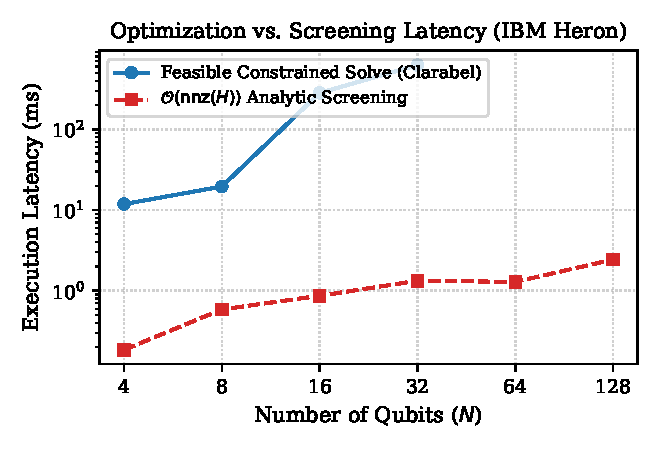
\includegraphics[width=0.92\columnwidth]{figures/observable_runtime_scaling.pdf}
\caption{Local solver times under a saved Heron calibration snapshot. The original absolute-target protocol has feasible solves only through 32 qubits; its 64- and 128-qubit timings measure analytic rejection, not optimization.}\label{fig:runtime}
\end{figure}

\begin{figure}[t]
\centering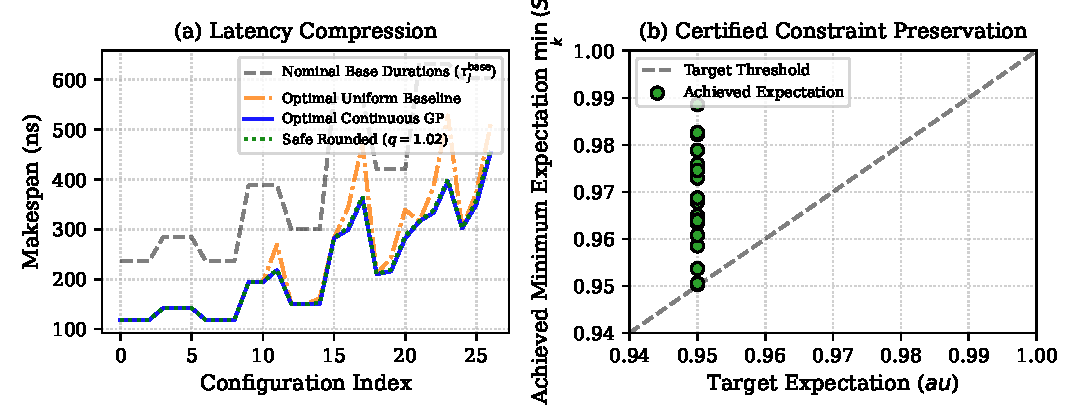
\includegraphics[width=\columnwidth]{figures/observable_makespan_fidelity.pdf}
\caption{Modeled performance using a saved Heron snapshot: (a) Latency compression showing makespan reduction across nominal calibrated base durations ($\tau_j^{\mathrm{base}}$) and the optimal uniform-duration baseline. (b) Certified preservation of operational expectation targets $\langle S_k \rangle \ge \tau$ after discrete log-grid rounding ($q=1.02$).}\label{fig:makespan_fidelity}
\end{figure}

\subsection{Feasible Solves Through 128 Qubits}
To measure solver behavior at larger sizes, we ran a separate, model-attainable protocol on 24 configurations at 32, 64, and 128 qubits (two families, two seeds, and assumed $\alpha\in\{0.5,0.8\}$). For each instance, let $e_\ell$ be the minimum generator expectation at the lower-duration vector and $e_{\min}$ the minimum expectation at the coordinatewise minimum-hazard vector. We set the target to $\sqrt{e_\ell e_{\min}}$ and require $e_\ell<\sqrt{e_\ell e_{\min}}<e_{\min}$. This deliberately selects a nontrivial feasible target using the same model; it is a solver stress test, not external noise validation. We compare with the earliest \emph{optimal uniform scaling} that satisfies that identical target. Targets vary by instance, so absolute fidelity levels are not comparable across sizes.

All 24 GP and direct-convex solves were feasible and their makespans agreed to a maximum relative difference below $3\times10^{-7}$. Table~\ref{tab:feasible_scale} reports descriptive medians of single-run wall time and modeled makespan reduction. The 128-qubit cases include up to 830 timed gates; their median observed solve time is 6.41~s. These runs address the earlier missing feasible large-scale solve, but do not establish linear scaling or physical speedup. The additional grid-rounding margin was not imposed in this study; a tightened margin may itself be infeasible or numerically difficult even when the original target is feasible.

\begin{table}[t]
\centering
\caption{Feasible model-based solves. Targets are chosen separately per instance from its assumed attainable range; times are single-run wall-clock observations, not hardware timings. Makespan reduction against the optimal uniform policy is reported separately for each assumed inverse-duration share $\alpha$ (median over families and seeds).}
\label{tab:feasible_scale}
\footnotesize
\begin{adjustbox}{max width=\columnwidth}
\begin{tabular}{rrrrrr}
\toprule
Qubits & $n$ & Gates & GP ms & Gain, $\alpha=0.5$ & Gain, $\alpha=0.8$ \\
\midrule
32 & 8 & 64--200 & 1166.3 & 14.9\% & 22.2\% \\
64 & 8 & 132--412 & 2954.1 & 18.0\% & 30.9\% \\
128 & 8 & 266--830 & 6413.8 & 18.0\% & 30.9\% \\
\bottomrule
\end{tabular}
\end{adjustbox}
\end{table}


\begin{figure}[t]
\centering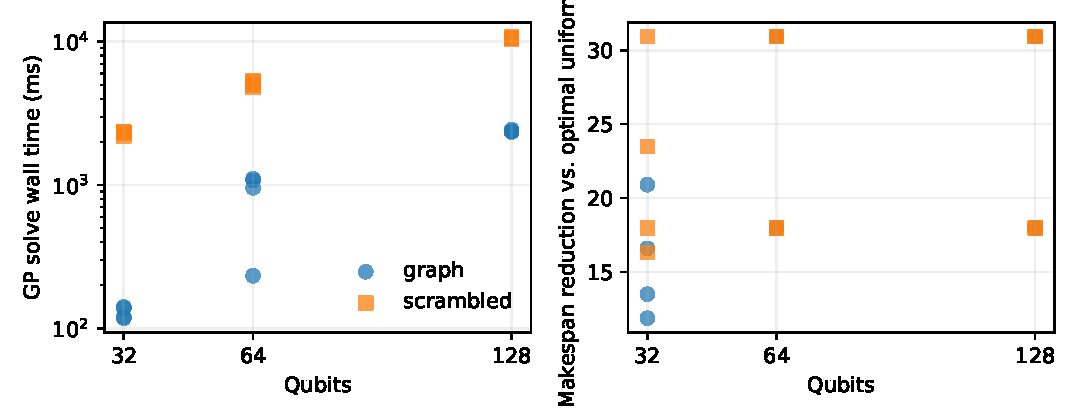
\includegraphics[width=\columnwidth]{figures/feasible_scale.pdf}
\caption{Model-attainable 32--128-qubit continuous solves. Each point is one local solve; the right panel compares with an optimal uniform policy under the same instance-specific target. Neither panel measures device execution.}\label{fig:feasible_scale}
\end{figure}

\paragraph{Per-instance reductions.}
The identical $24.5\%$ medians at 64 and 128 qubits in Table~\ref{tab:feasible_scale} are an artifact of taking a median. No instance attains $24.5\%$: at both sizes, the eight reductions split into four at $17.98\%$ (all $\alpha=0.5$ instances) and four at $30.92\%$ (all $\alpha=0.8$ instances), and the median of an even-sized two-cluster sample is their midpoint. The split is set by the assumed inverse-duration share $\alpha$, not by circuit family or topology. We therefore report per-instance and per-$\alpha$ values rather than a pooled median, and make no claim of a structural compression limit.

\subsection{Multi-Circuit Matched-Deadline Evaluation and Unconstrained Benchmark}
\begin{table}[t]
\caption{Characterized MILP versus adapted published slack (48 cases per regime). Fidelity changes are percentage points (pp); intervals are exploratory cluster bootstraps.}\label{tab:physical}
\centering\small\setlength{\tabcolsep}{4pt}
\begin{tabular}{lrrrr}\toprule
Regime & Mean pp & Interval & Regressions & Latency \%\\\midrule
Low & -0.008 & [-0.02,0.00] & 16 & 0.05\\
Balanced & 3.966 & [3.10,4.86] & 0 & 32.55\\
High & 15.341 & [9.88,20.67] & 0 & 216.97\\
\bottomrule\end{tabular}\end{table}


Table~\ref{tab:physical} and Figure~\ref{fig:gains} report an initial \emph{unconstrained slack-stealing benchmark} where circuit makespans were permitted to expand (incurring $+32.55\%$ latency in Balanced and $+216.97\%$ in High Drive) to accommodate longer, decoherence-limited gates on non-critical paths. The Lussi et al. scheduler is our adaptation of the published heuristic \cite{lussi}, not an independently supplied implementation. In that unconstrained benchmark, the Low Drive row exhibits a slight regression of $-0.008$ pp ($[-0.02, 0.00]$, 16 regressions) because minimal off-critical slack existed.

In contrast, Table~\ref{tab:matched_deadlines} presents the primary \emph{matched-deadline experiment} across 48 multi-qubit circuits (6 distinct families: Grover, Mirror, QAOA, QFT, Random Pauli, and VQE Ansatz; 4 random seeds each; 2 and 3 qubits), where makespans are strictly fixed to match the fastest ASAP baseline. Stratified 5,000-replicate bootstrap confidence intervals quantify statistical sampling variability.

\begin{table}[t]
\caption{Matched-deadline fidelity comparison across 48 multi-qubit circuits (6 families, 4 seeds, qubits 2--3) under strictly fixed makespan equal to the fastest baseline. Fidelity changes are reported in percentage points (pp). Intervals are stratified 5,000-replicate bootstrap 95\% confidence intervals.}\label{tab:matched_deadlines}
\centering\footnotesize\setlength{\tabcolsep}{1.8pt}
\begin{tabular}{lccccc}\toprule
Regime & Feas./Total & Mean pp & 95\% Bootstrap CI & Regr. & Median pp \\\midrule
Low Drive  & 47/48$^*$ & -0.0096 & [-0.0152, -0.0045] & 17 & 0.0000 \\
Balanced   & 48/48     & +0.0258 & [+0.0155, +0.0374] & 1  & 0.0000 \\
High Drive & 48/48     & +0.0081 & [+0.0026, +0.0141] & 5  & 0.0000 \\
\bottomrule
\end{tabular}\\[2pt]
\parbox{0.96\columnwidth}{\scriptsize $^*$One circuit (\texttt{qaoa\_3\_103}) is HiGHS solver infeasible under the fastest matched deadline.}
\end{table}

Under matched deadlines, Low Drive shows a statistically significant regression of $-0.0096$ pp ($[-0.0152, -0.0045]$ pp, 17 regressions out of 47 feasible cases), while Balanced yields $+0.0258$ pp ($[+0.0155, +0.0374]$ pp, 1 regression) and High Drive yields $+0.0081$ pp ($[+0.0026, +0.0141]$ pp, 5 regressions). Crucially, the median gain across all three regimes is exactly $0.0000$ pp. Under tight matched deadlines, non-critical slack is minimal; any duration elongation on near-critical gates risks increasing cumulative idling or violating precedence. Hence, the gate-duration-only method of this section does not deliver general physical fidelity improvements at fixed latency; the joint timing-and-decoupling allocation of Section~\ref{sec:framework} is evaluated separately below.

\begin{figure}[t]
\centering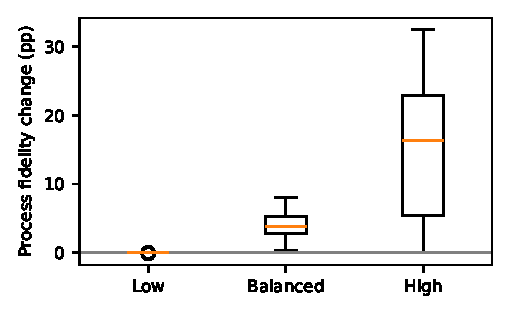
\includegraphics[width=0.88\columnwidth]{figures/physical_gains.pdf}
\caption{Paired process-fidelity changes against adapted published slack scheduling \cite{lussi} on the same simulated library, showing modeled fidelity and latency trade-offs; the matched-deadline result is reported in Table~\ref{tab:matched_deadlines}.}\label{fig:gains}
\end{figure}

\begin{figure}[t]
\centering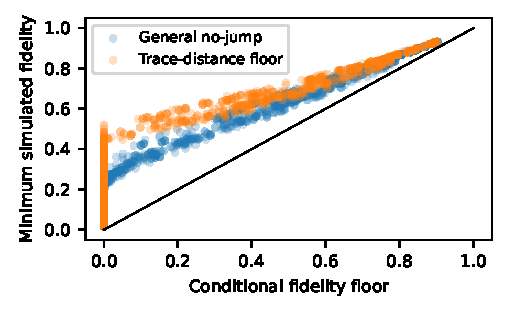
\includegraphics[width=0.88\columnwidth]{figures/physical_certificates.pdf}
\caption{General-jump certificate coverage. All simulated fidelities lie strictly above the analytical theoretical fidelity floors, checking implementation consistency with the assumed Lindblad model; this is not external physical validation.}\label{fig:cert}
\end{figure}

\subsection{Model-Fit Tests and Noise Misspecification Stress Tests}
We tested the assumed inverse-plus-linear law on a publicly deposited experimental single-qubit randomized-benchmarking (RB) duration sweep by Hyypp\"a \emph{et al.}~\cite{hyyppa_data}. Its Figure~3a archive provides measured mean error per gate, one-standard-deviation uncertainties, and durations for four calibrated pulse families. For each family, durations were sorted and alternating points allocated to fitting and held-out evaluation (54 points overall; 25 held out). Nonnegative weighted least squares fitted $e(t)=A/t+Gt$ on the fit points using inverse reported variance. Table~\ref{tab:law_comparison} and Figure~\ref{fig:measured_duration} report the held-out results. The law beats a constant-error predictor in mean absolute error for each family, but squared residuals measured in reported standard deviations are large (mean squared residuals range from 23 to 83 against reported variance). Thus its qualitative trade-off can describe these measurements while its two-parameter form does not adequately explain their reported uncertainty. An exploratory inverse-square variant ($A/t^2+Gt$) does not resolve this discrepancy. Presenting these as negative results emphasizes that the continuous GP model is an idealized engineering abstraction.

\begin{table}[t]
\centering\caption{Exploratory leave-one-duration-out error-law comparison. MAE columns are in units of $10^{-4}$; RMS is the root mean squared residual divided by source-reported one-sigma uncertainty. The inverse-square candidate was chosen after viewing earlier holdout data.}\label{tab:law_comparison}
\begin{tabular}{lccc}\hline
Pulse family & $1/t+t$ MAE & $1/t^2+t$ MAE & $1/t^2+t$ RMS\\\hline
FAST DRAG-L & 0.448 & 0.372 & 4.69\\
HD DRAG-L & 1.345 & 1.153 & 14.74\\
Cosine DRAG-L & 4.878 & 4.524 & 10.98\\
Cosine DRAG-P & 6.309 & 5.977 & 8.58\\
\hline\end{tabular}
\end{table}


\paragraph{Measured finite-library decision audit.}
To test whether lower prediction error improves an actual choice, we fitted each law on the marked training durations and required it to select from the \emph{same withheld measured duration options} within each pulse family. We also evaluated shape-preserving piecewise-cubic interpolation (PCHIP) as an exploratory empirical alternative. Table~\ref{tab:choice_audit} reports regret relative to the lowest reported RB error among withheld options. The two GP-compatible laws selected the same option in all four families. PCHIP selected the lowest observed option in three families and missed by $4.97\times10^{-6}$ error per gate in HD DRAG-L; the inverse-power laws selected the lowest option in HD DRAG-L but incurred larger regret in FAST DRAG-L and Cosine DRAG-P. Thus a better \emph{measured} duration choice is possible on this retrospective library, but it comes from an empirical finite-library predictor, not the proposed inverse-power GP law.

\begin{table}[t]
\centering\caption{Exploratory measured finite-library duration choices. Entries are measured regret against the lowest-error withheld option, in $10^{-5}$ RB error per gate. The empirical interpolator was examined after earlier law results; these are not prospective gains.}\label{tab:choice_audit}
\begin{tabular}{lccc}\hline
Pulse family & $1/t+t$ & $1/t^2+t$ & PCHIP\\\hline
FAST DRAG-L & 3.076 & 3.076 & 0.000\\
HD DRAG-L & 0.000 & 0.000 & 0.497\\
Cosine DRAG-L & 0.000 & 0.000 & 0.000\\
Cosine DRAG-P & 3.452 & 3.452 & 0.000\\
\hline\end{tabular}
\end{table}


\begin{figure*}[t]
\centering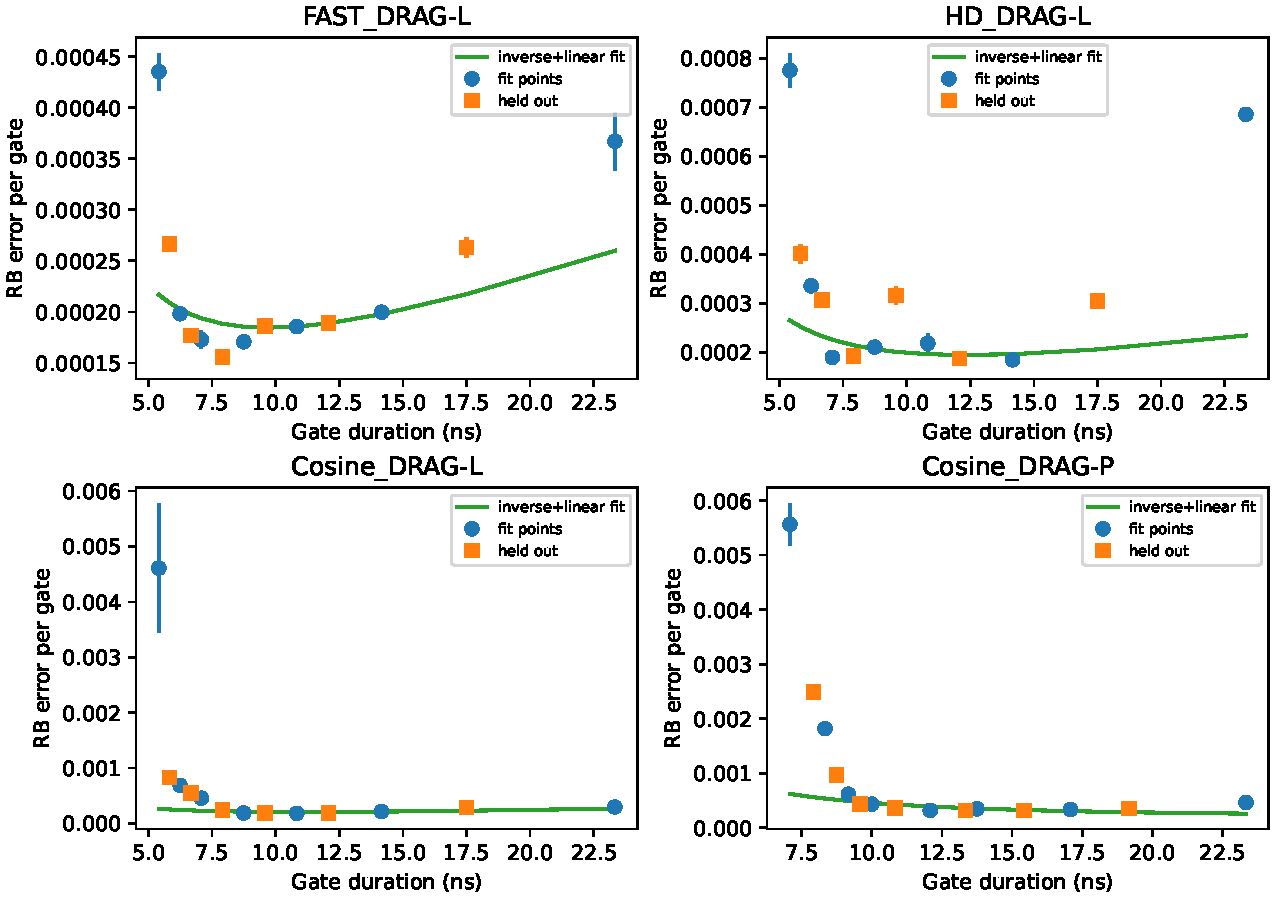
\includegraphics[width=0.78\textwidth]{figures/measured_duration.pdf}
\caption{Published experimental single-qubit RB gate error versus duration for four pulse families \cite{hyyppa_data}. Circles fit the nonnegative inverse-plus-linear law; squares are held out. Error bars show source-reported one-standard-deviation uncertainties.}\label{fig:measured_duration}
\end{figure*}

\paragraph{Structural Noise Model Misspecification Stress Test.}
To test the sensitivity of the GP schedule to structural model misspecification, we evaluated continuous allocations optimized under the declared inverse-linear model ($a/\tau + \gamma\tau$) when the underlying physical error instead follows an inverse-quadratic law $\epsilon(\tau) \propto 1/\tau^2$ (characteristic of non-adiabatic state leakage or higher-order drive distortions). As documented in Table~\ref{tab:noise_misspecification}, in all 6 evaluated benchmark circuits (100\%), the GP-chosen durations produced strictly higher physical error than the uniform base schedule. This shows that GP duration allocation is fragile under structural model misspecification. A rerun (Table~\ref{tab:c4a}) locates the cause: the inverse-square law used here is not unit-matched to the declared law at nominal duration, so it lies outside any hull of matched laws. On 30 law--circuit pairs inside the hull (inverse, unit-matched inverse-square, and their mixtures), no GP schedule is worse than the baseline. Declaring this law in the dominance set of Theorem~\ref{th:dominance} removes every regression, at a cost of at most 0.3 percentage points of the improvement on the declared law.

\begin{table}[t]
\centering\caption{Noise model misspecification stress test: evaluating continuous schedules optimized under the standard $1/\tau$ law against an alternative quadratic physical error model $\epsilon \propto 1/\tau^2$. Error rates are reported per circuit.}\label{tab:noise_misspecification}
\footnotesize\setlength{\tabcolsep}{3pt}
\begin{tabular}{lcccc}\toprule
Circuit & Base Error & GP Error & Difference & Outcome \\\midrule
\texttt{qft\_3}    & 0.0325 & 0.0355 & +0.0031 & Worse (Regression) \\
\texttt{qft\_4}    & 0.0674 & 0.0765 & +0.0091 & Worse (Regression) \\
\texttt{grover\_3} & 0.0650 & 0.0689 & +0.0039 & Worse (Regression) \\
\texttt{grover\_4} & 0.1924 & 0.2112 & +0.0188 & Worse (Regression) \\
\texttt{vqe\_3}    & 0.0200 & 0.0224 & +0.0024 & Worse (Regression) \\
\texttt{vqe\_4}    & 0.0297 & 0.0318 & +0.0021 & Worse (Regression) \\\bottomrule
\end{tabular}\\[2pt]
\parbox{0.96\columnwidth}{\scriptsize Across all 6 evaluated circuits (100\%), GP durations yield higher physical infidelity.}
\end{table}

\paragraph{Calibration Pairs and Idle-Noise Scheduling Stress Test.}
We extracted 566 reported gate-error/duration pairs for \texttt{sx}, \texttt{x}, and \texttt{cz} from the saved \emph{ibm\_torino} fake-backend calibration file. These are cross-sectional entries across gates and locations, sometimes with different parameter timestamps; they are not repeated measurements of one gate under controlled duration changes. Figure~\ref{fig:schedule_noise}(a) displays the pairs descriptively. Fitting $a/t+\gamma t$ to this scatter would confound qubit, gate type, and calibration state, so no duration-response coefficients were inferred.

For a three-qubit native Clifford circuit, Qiskit's \texttt{ASAPScheduleAnalysis} and \texttt{ALAPScheduleAnalysis} were each followed by \texttt{PadDelay} or \texttt{PadDynamicalDecoupling} with two $X$ pulses. All four schedules have the same 168-ns makespan and ideal output state. We independently propagated the density matrix under gate-local anisotropic Pauli errors, idle amplitude damping and dephasing, and, in one scenario, a Gaussian shot-static $Z$ detuning acting during idles. Seven-node Gauss--Hermite quadrature per qubit integrated the static detuning. Table~\ref{tab:schedule_noise} gives ideal-state fidelities. Under Markovian $Z$-biased noise, DD adds faulty gates and lowers the ASAP fidelity; under shot-static detuning, ASAP+DD refocuses the long idle and improves it.

\begin{table}[t]
\centering\caption{Matched 168-ns Qiskit scheduling baselines; simulated ideal-state fidelity (no hardware jobs).}\label{tab:schedule_noise}
\begin{tabular}{lccc}\hline
Policy & Isotropic & $Z$-biased & Static $Z$ + biased\\\hline
ASAP & 0.996804 & 0.995908 & 0.696027\\
ALAP & 0.997087 & 0.996191 & 0.882678\\
ASAP+DD & 0.996215 & 0.994426 & 0.994426\\
ALAP+DD & 0.996281 & 0.995982 & 0.882493\\\hline
\end{tabular}
\end{table}

\begin{figure*}[t]
\centering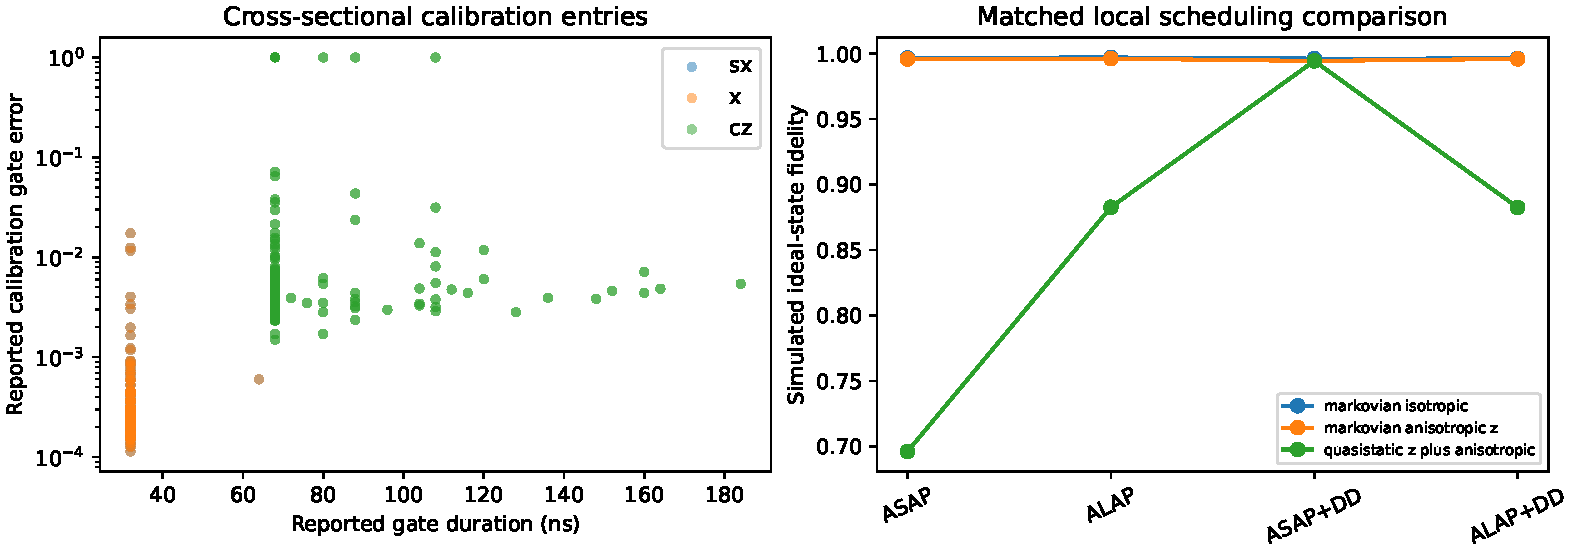
\includegraphics[width=0.88\textwidth]{figures/schedule_noise.pdf}
\caption{Left: cross-sectional reported calibration pairs from a cached fake-backend file, not a controlled duration sweep. Right: matched-makespan local density-matrix simulation under three declared noise scenarios.}\label{fig:schedule_noise}
\end{figure*}

\paragraph{Note on Table Consistency Across Evaluations.}
In Table~\ref{tab:schedule_noise}, Qiskit ASAP under static detuning reports simulated fidelity $0.6960$, whereas in Table~\ref{tab:direct_matched} below it reports $0.6948$. The two evaluations evaluate different circuits: Table~\ref{tab:schedule_noise} evaluates a 3-qubit Clifford benchmark with nominal backend gate delays, while Table~\ref{tab:direct_matched} evaluates a five-gate circuit with explicit delay padding and per-qubit phase tracking during delays. Across both evaluations, the slight difference stems from circuit gate count and delay intervals; both demonstrate massive dephasing without dynamical decoupling.

\subsection{Direct Equal-Deadline Comparison with Qiskit Scheduling}
We next optimized the durations of the same five-gate, three-qubit circuit with the declared inverse-power law, using $p=1$ or $p=2$, a drive-error share $\alpha=0.8$, duration bounds $[0.5,1.5]$ times each nominal duration, and a 168-ns critical-path deadline. Nominal durations and errors came from the saved \emph{ibm\_torino} snapshot; the duration dependence and $\alpha$ are \emph{assumed}, not calibrated. Each GP vector was placed ASAP or ALAP and padded to the common deadline. We compared it directly with Qiskit's ASAP/ALAP passes with either delay padding or two-$X$ DD padding. All eight policies preserve the logical operation and meet 168~ns; the DD variants add two $X$ gates. The GP variants require hypothetical alternate-duration native pulses, whereas Qiskit schedules the snapshot's fixed nominal gates.

Table~\ref{tab:direct_matched} reports deterministic simulated ideal-state fidelity. Under the aligned $p=1$ Markovian model, GP-$p=1$ ALAP reaches 0.993483 versus Qiskit ALAP's 0.993162, a small absolute gain. However, because the GP solver optimizes the exact mathematical error law evaluated, this gain ($\sim 3\times 10^{-4}$) is largely a self-prediction of the aligned model. When evaluated against an unoptimized flat-error control, the gain drops by an order of magnitude to $\sim 4\times 10^{-5}$, consisting solely of minor idle placement differences. Under shot-static detuning, Qiskit ASAP+DD reaches 0.993448 while the best GP-only schedule drops to 0.938164. This rank reversal confirms that duration allocation without dynamical decoupling fails under unmodeled low-frequency dephasing.

\begin{table*}[t]
\centering\caption{Direct local comparison at a common 168-ns deadline: simulated ideal-state fidelity under declared hypothetical duration laws and noise models. No hardware jobs or measured duration-response curves.}\label{tab:direct_matched}
\begin{tabular}{lcccc}\hline
Policy & $p=1$, isotropic & $p=2$, $Z$ biased & Flat, $Z$ biased & $p=1$, static $Z$\\\hline
GP $p=1$ ASAP & 0.993289 & 0.994205 & 0.994041 & 0.821760\\
GP $p=1$ ALAP & 0.993483 & 0.994399 & 0.994235 & 0.932671\\
GP $p=2$ ASAP & 0.993278 & 0.994357 & 0.994044 & 0.814316\\
GP $p=2$ ALAP & 0.993474 & 0.994553 & 0.994239 & 0.938164\\
Qiskit ASAP & 0.992880 & 0.993920 & 0.993920 & 0.694797\\
Qiskit ALAP & 0.993162 & 0.994203 & 0.994203 & 0.881003\\
Qiskit ASAP+DD & 0.992584 & 0.993448 & 0.993448 & 0.993448\\
Qiskit ALAP+DD & 0.992650 & 0.994042 & 0.994042 & 0.880861\\\hline
\end{tabular}
\end{table*}

\begin{figure*}[t]
\centering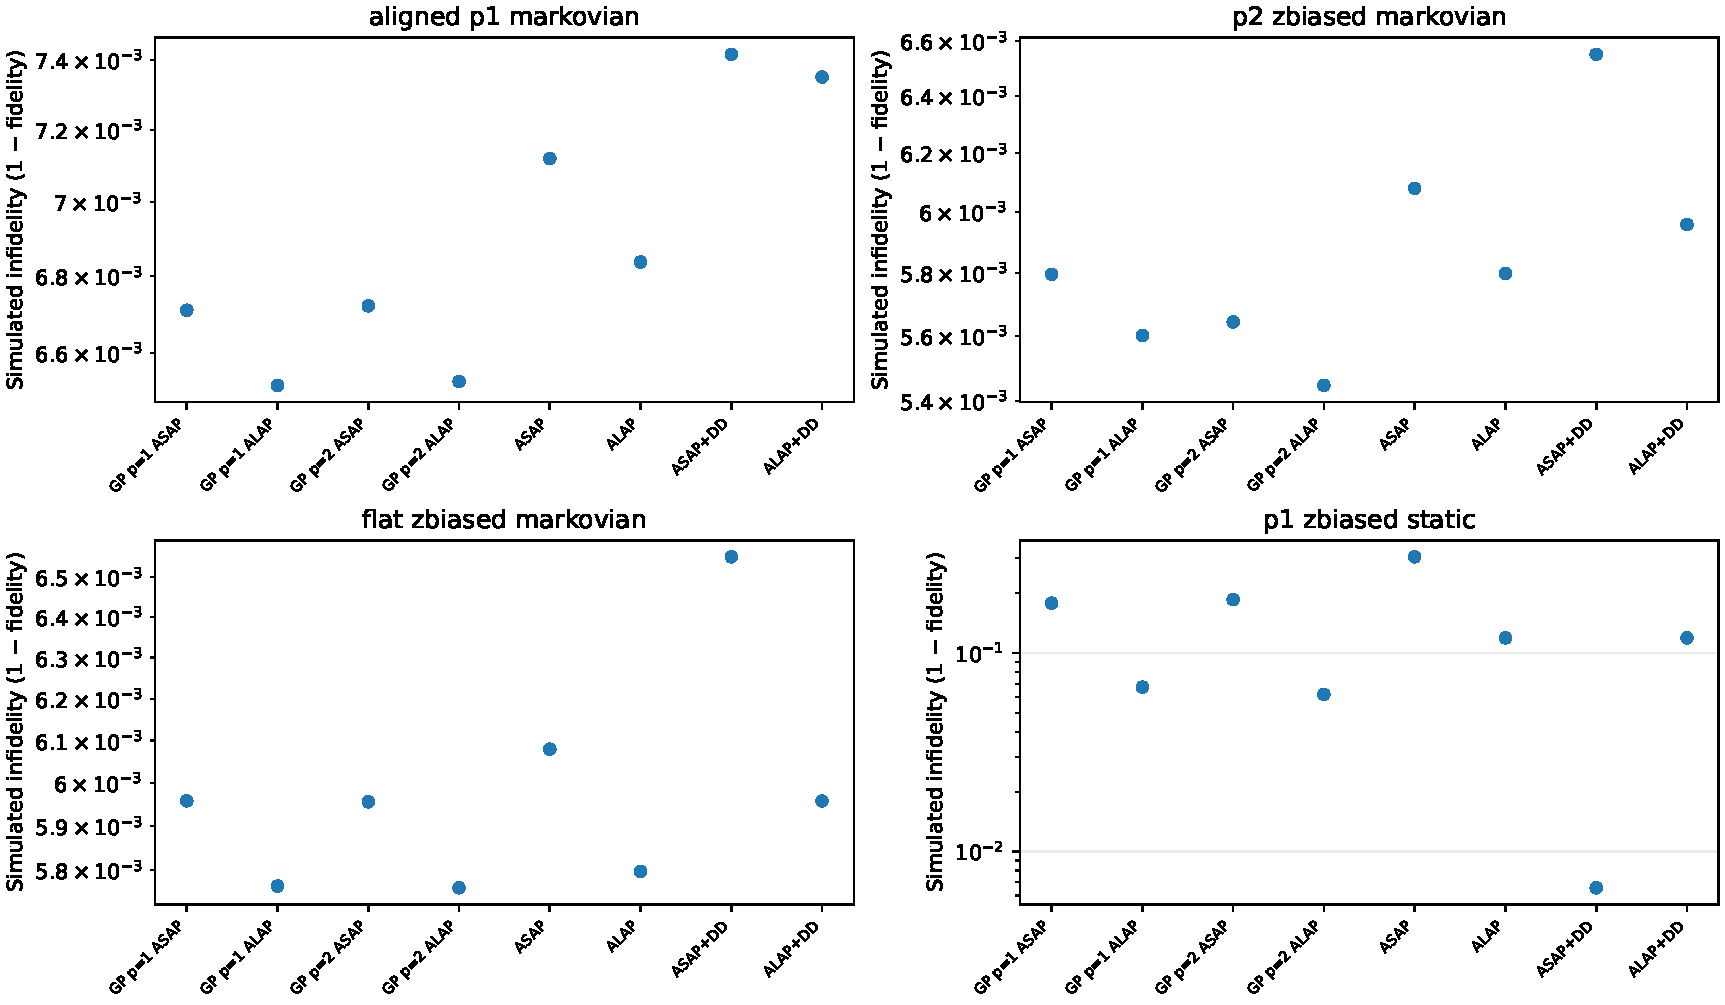
\includegraphics[width=0.95\textwidth]{figures/direct_matched.pdf}
\caption{Simulated infidelity ($1-F$; logarithmic axis) for the eight policies in Table~\ref{tab:direct_matched}. The horizontal positions are categorical. The static-detuning case exposes a large rank reversal favoring DD.}\label{fig:direct_matched}
\end{figure*}

\subsection{Physical Hardware Gate-Choice Experiment on Heron: Qualitative Motivation for Duration-Aware Compilation}
To examine whether physical pulse durations impact decoherence dynamics on quantum hardware, we conducted an experimental study on \texttt{ibm\_marrakesh}. This experiment provides qualitative motivation for duration-aware compilation, rather than empirical support for the continuous GP formulation. On \texttt{ibm\_marrakesh}, the backend's published instruction set (its Qiskit \texttt{Target}) exposes two implementations of the logical X gate on all 156 qubits: native \texttt{x} ($36$~ns) and an extended-duration bit flip \texttt{xslow} ($1{,}000$~ns). We used both on physical qubits 0 and 1. A $1{,}000$-ns gate is approximately $28\times$ longer than the $36$-ns base duration, lying far outside the continuous range $[0.5, 1.5]\times 36$~ns ($18\text{--}54$~ns) optimized by the GP formulation. The backend reports the \emph{same} nominal error for both gates, providing no calibrated duration dependence.

We submitted an exploratory characterization job (\texttt{db4ob04lf4us73c31490}): sequences of 0, 8, 32, or 64 X gates in X- and Z-basis return experiments on both qubits. At 32 gates on qubit 1 in the X basis, slow X exceeded the equal-duration padded control by 0.0120 across three blocks, but the shot-only 95\% interval included zero. We selected physical qubit 1 for a separately frozen holdout; this training-guided selection restricts generality.

The held-out job (\texttt{db4ocm2mb58s7389fnag}) evaluated untested lengths of 16 and 48 X gates, both bases, and three randomized blocks of 2,048 shots (6,144 shots total per policy). It compared slow X, distributed X-plus-delay padding, fast X followed by one tail delay, and the latter processed by Qiskit's ALAP analysis with two-X dynamical decoupling. All four implementations had identical ideal unitaries and nominal total durations ($48{,}000$~ns at 48 gates); the two-X DD gate time was compensated in its tail delay.

\begin{table}[t]
\centering\caption{Held-out Heron native-X implementation comparison at 48 logical X gates on physical qubit 1. Entries are observed return-to-zero frequencies from three randomized blocks (6,144 shots per policy and basis), not average gate fidelities. Every policy has the same nominal duration.}\label{tab:x_duration_hardware}
\begin{tabular}{lcc}\hline
Policy & X-basis return & Z-basis return\\\hline
Slow X & 0.9010 & 0.8296\\
Fast X, distributed delays & 0.8826 & 0.8013\\
Fast X, tail delay & 0.3052 & 0.9849\\
Fast X, two-X DD tail & 0.8586 & 0.8753\\\hline
\end{tabular}
\end{table}

\begin{figure}[t]
\centering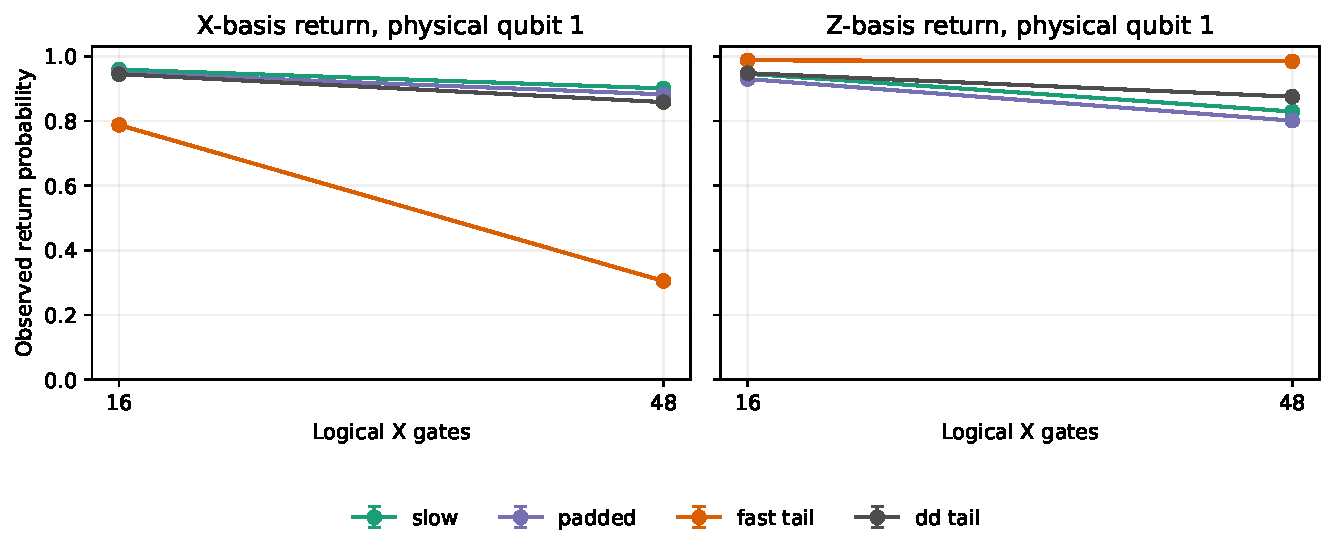
\includegraphics[width=\columnwidth]{figures/ibm_marrakesh_x_duration_holdout_2026-10-10.pdf}
\caption{Held-out physical X-duration comparison at equal nominal total durations. Error bars are shot-only 95\% normal intervals and exclude device drift. The reversal between X- and Z-basis return makes a single scalar gate-error rate inadequate for these sequences.}\label{fig:x_duration_hardware}
\end{figure}

\paragraph{Failure Mode of Tail Delay.}
As reported in Table~\ref{tab:x_duration_hardware} and Fig.~\ref{fig:x_duration_hardware}, the `Fast X, tail delay' baseline suffers a catastrophic failure mode in the X basis, collapsing to return probability $0.3052$. This collapse suggests severe accumulated coherent detuning and low-frequency dephasing during the unrefocused $46{,}272$-ns tail idle interval. In contrast, continuously driving the qubit throughout the $1{,}000$-ns slow X pulses suppressed this dephasing ($P(0) = 0.9010$).

\paragraph{Thin Statistics and Observable-Dependent Reversal.}
The headline $4.25$ percentage point gain for slow X over two-X DD ($0.9010$ vs $0.8586$) has a paired interval from only three randomized blocks ($0.0288\text{--}0.0561$). Three blocks do not establish temporal or calibration robustness. Crucially, in the Z basis, slow X is worse than two-X DD ($0.8296$ vs $0.8753$, a $-0.0457$ deficit) and worse than fast X with tail delay ($0.9849$). A fair summary is that the preferred implementation policy depends entirely on the measured observable and basis.

\paragraph{Selection Issue and Internal Model Critique.}
Physical qubit 1 and the X basis were selected post-training; repeating on unselected qubits (qubits 0 and 2) across distinct calibration cycles is necessary to decouple pulse physics from transient calibration artifacts. Most importantly, the sharp basis-dependent rank reversal provides an internal model critique: it directly falsifies the single-scalar, isotropic post-gate Pauli noise model that underlies the GP formulation. Because no GP optimizer chose the physical circuit, this experiment demonstrates that pulse duration choices alter hardware decoherence dynamics, but does not validate the GP timing algorithm. GP-selected schedules are tested on hardware in the pre-registered decoupling study below.

\subsection{Independent Time-Correlated Simulator}
The following studies never evaluate a schedule with its own optimization model. A batched density-matrix simulator applies, per qubit, classical detuning noise (a quasi-static Gaussian offset plus a spectral sum approximating $S(f)\propto f^{-\beta}$, with common random numbers across policies), Markovian or exact non-unital amplitude damping, duration-dependent Pauli gate errors, and imperfect DD pulses. It reproduces analytic Ramsey decay and echo refocusing in unit tests. GP models are fitted only from simulated single-qubit spectroscopy, mirroring the hardware protocol below.

\subsection{Joint Timing and Decoupling (Section~\ref{sec:framework})}
At a deadline equal to the nominal ASAP makespan, across five noise spectra and four circuits (Table~\ref{tab:c2}), joint allocation with cross-window protection beats the best of ASAP, ALAP, ALAP+XX and ALAP+XY4 in \CTwoWins{} of \CTwoCases{} cases and is significantly worse in \CTwoLosses{} (median \CTwoMedian$\times10^{-4}$). The model ranks policies with median Spearman correlation \CTwoRank{} against the simulator. Three findings qualify this.
\begin{itemize}
\item Most of the gain comes from stretching gates into slack (Corollary~\ref{cor:threshold}). With native fixed durations, the hardware-executable setting, the GP wins \CTwoFixedWins{} and loses \CTwoFixedLosses{} cases.
\item The largest losses occur on a repetition-code circuit under quasi-static or $1/f$ noise, where phase accumulates coherently across idle windows. Cross-window protection (Proposition~\ref{prop:state}) reduces that loss from $236\times10^{-4}$ to $57\times10^{-4}$.
\item A first evaluation protocol charged decoherence during gates twice. Under it the GP won \CTwoVoneWins{} and lost \CTwoVoneLosses{} cases (rank correlation \CTwoVoneRank{}). We corrected the protocol and report both versions in the repository.
\end{itemize}
\begin{table*}[t]
\centering
\caption{Joint timing and decoupling allocation at matched makespan: simulated state-fidelity change against the best standard policy (ASAP, ALAP, ALAP+XX, ALAP+XY4), in units of $10^{-4}$ with paired standard errors over common noise realisations. Columns: the earlier gate-only GP; cross-window GP-DD with native (fixed) durations, which is hardware-executable; and cross-window GP-DD with duration control. Models are fitted only from simulated single-qubit spectroscopy.}\label{tab:c2}
\footnotesize
\begin{adjustbox}{max width=0.95\textwidth}
\begin{tabular}{llcrrrr}
\toprule
Noise & Circuit & Best std. & Gate-only GP & GP-DD fixed $\tau$ & GP-DD joint & Pulses \\
\midrule
one\_over\_f & ghz6\_chain & asap & +0.3 $\pm$ 0.1 & -0.0 $\pm$ 0.0 & -0.9 $\pm$ 0.1 & 0 \\
one\_over\_f & mirror5\_with\_block & alap\_xx & -92.9 $\pm$ 7.0 & -34.5 $\pm$ 2.5 & +18.8 $\pm$ 5.0 & 2 \\
one\_over\_f & qft4\_native & alap & +15.7 $\pm$ 0.6 & -2.8 $\pm$ 0.3 & +25.2 $\pm$ 0.3 & 0 \\
one\_over\_f & rep3\_two\_cycles & alap\_xx & -346.0 $\pm$ 29.2 & -16.7 $\pm$ 3.3 & -14.9 $\pm$ 3.4 & 10 \\
one\_over\_f2 & ghz6\_chain & asap & +0.8 $\pm$ 0.0 & -0.0 $\pm$ 0.0 & -0.8 $\pm$ 0.0 & 0 \\
one\_over\_f2 & mirror5\_with\_block & alap\_xx & +43.3 $\pm$ 2.1 & +13.0 $\pm$ 1.6 & +100.6 $\pm$ 1.6 & 0 \\
one\_over\_f2 & qft4\_native & alap & +23.8 $\pm$ 0.1 & -0.2 $\pm$ 0.1 & +30.2 $\pm$ 0.1 & 0 \\
one\_over\_f2 & rep3\_two\_cycles & alap\_xx & -55.4 $\pm$ 7.9 & -4.1 $\pm$ 2.3 & -1.0 $\pm$ 2.4 & 6 \\
one\_over\_f\_bad\_pulses & ghz6\_chain & asap & +0.3 $\pm$ 0.1 & -0.0 $\pm$ 0.0 & -3.3 $\pm$ 0.3 & 0 \\
one\_over\_f\_bad\_pulses & mirror5\_with\_block & asap & +20.1 $\pm$ 0.3 & +65.7 $\pm$ 4.0 & +146.6 $\pm$ 4.2 & 0 \\
one\_over\_f\_bad\_pulses & qft4\_native & alap & +10.1 $\pm$ 0.6 & -2.8 $\pm$ 0.3 & +6.7 $\pm$ 0.3 & 0 \\
one\_over\_f\_bad\_pulses & rep3\_two\_cycles & asap & +1.0 $\pm$ 0.4 & -0.0 $\pm$ 0.0 & +1.5 $\pm$ 0.5 & 0 \\
quasi\_static & ghz6\_chain & asap & +0.6 $\pm$ 0.0 & -0.0 $\pm$ 0.0 & -0.8 $\pm$ 0.1 & 0 \\
quasi\_static & mirror5\_with\_block & alap\_xx & -33.9 $\pm$ 4.9 & -26.5 $\pm$ 3.0 & +54.1 $\pm$ 3.9 & 0 \\
quasi\_static & qft4\_native & alap & +20.2 $\pm$ 0.4 & -1.3 $\pm$ 0.2 & +28.5 $\pm$ 0.2 & 0 \\
quasi\_static & rep3\_two\_cycles & alap\_xx & -235.9 $\pm$ 22.9 & -58.2 $\pm$ 6.9 & -57.4 $\pm$ 7.1 & 6 \\
white\_markov & ghz6\_chain & asap & -0.6 $\pm$ 0.0 & -0.0 $\pm$ 0.0 & -2.0 $\pm$ 0.0 & 0 \\
white\_markov & mirror5\_with\_block & asap & +78.6 $\pm$ 0.0 & +19.4 $\pm$ 0.0 & +87.6 $\pm$ 0.0 & 0 \\
white\_markov & qft4\_native & alap & +15.1 $\pm$ 0.0 & -14.3 $\pm$ 0.0 & +10.3 $\pm$ 0.0 & 0 \\
white\_markov & rep3\_two\_cycles & asap & +3.4 $\pm$ 0.0 & -0.0 $\pm$ 0.0 & -2.2 $\pm$ 0.0 & 0 \\
\bottomrule
\end{tabular}
\end{adjustbox}
\end{table*}


Under exact amplitude damping with fixed durations (Table~\ref{tab:c5b}), the state-aware allocation places pulses only on qubits idling in $|1\rangle$, where a balanced block halves $T_1$ exposure, and beats blanket XX by $20$--$70\times10^{-4}$ with fewer pulses.

\begin{table*}[t]
\centering
\caption{State-aware and cross-window DD allocation under exact amplitude damping (fidelity change, $10^{-4}$, paired s.e.): state-aware vs state-blind GP-DD; state-aware vs ALAP+XX; cross-window (correlated) GP-DD vs ALAP+XX; pulses used (correlated/XX).}\label{tab:c5b}
\footnotesize
\begin{adjustbox}{max width=0.95\textwidth}
\begin{tabular}{llrrrr}
\toprule
Noise & Circuit & Aware$-$blind & Aware$-$XX & Correlated$-$XX & Pulses \\
\midrule
t1\_dominated & excited\_idle\_chain & +8.6 $\pm$ 0.0 & +70.3 $\pm$ 0.0 & +70.3 $\pm$ 0.0 & 2/6 \\
t1\_dominated & ghz5\_with\_ancilla\_wait & +0.0 $\pm$ 0.0 & +23.5 $\pm$ 0.0 & +23.5 $\pm$ 0.0 & 0/8 \\
t1\_dominated & rep3\_two\_cycles & +0.0 $\pm$ 0.0 & +57.4 $\pm$ 0.0 & +57.4 $\pm$ 0.0 & 0/16 \\
t1\_plus\_one\_over\_f & excited\_idle\_chain & +8.6 $\pm$ 0.0 & +70.2 $\pm$ 0.0 & +70.2 $\pm$ 0.0 & 2/6 \\
t1\_plus\_one\_over\_f & ghz5\_with\_ancilla\_wait & +0.0 $\pm$ 0.0 & +19.8 $\pm$ 0.4 & +19.8 $\pm$ 0.4 & 0/8 \\
t1\_plus\_one\_over\_f & rep3\_two\_cycles & +0.0 $\pm$ 0.0 & -93.5 $\pm$ 16.7 & -11.8 $\pm$ 5.7 & 6/16 \\
t1\_plus\_quasi\_static & excited\_idle\_chain & +8.6 $\pm$ 0.0 & +70.2 $\pm$ 0.0 & +70.2 $\pm$ 0.0 & 2/6 \\
t1\_plus\_quasi\_static & ghz5\_with\_ancilla\_wait & -0.0 $\pm$ 0.0 & +20.8 $\pm$ 0.3 & +20.8 $\pm$ 0.3 & 0/8 \\
t1\_plus\_quasi\_static & rep3\_two\_cycles & -0.0 $\pm$ 0.0 & -59.3 $\pm$ 12.1 & +1.5 $\pm$ 3.5 & 6/16 \\
\bottomrule
\end{tabular}
\end{adjustbox}
\end{table*}


\begin{figure*}[t]
\centering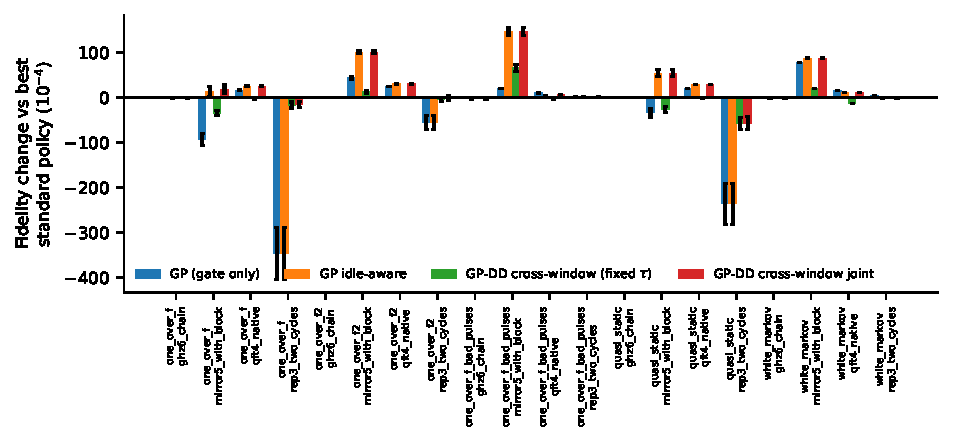
\includegraphics[width=0.95\textwidth]{figures/novelty_c2_dd_gp.pdf}
\caption{Simulated fidelity change against the best standard schedule per noise scenario and circuit (error bars: two paired standard errors).}\label{fig:c2}
\end{figure*}

\subsection{Runtime-Optimal PEC, Robustness, Anisotropy, and Scale}
\paragraph{Runtime (Table~\ref{tab:c3}).} Over 32 snapshot-anchored Clifford workloads, the convex optimum beats nominal, fastest, error-optimal and optimal-uniform durations in every case. The median QPU-time saving is \CThreeZero\% without repetition overhead, \CThreeFive\% at 5\,$\mu$s, and \CThreeIBM\% at IBM's default 250\,$\mu$s, as Theorem~\ref{th:runtime} predicts. These scheduling savings compound with overhead reductions obtained by other means \cite{scheiber2025,fischer2026}. Pauli-frame PEC sampling confirms unbiasedness and the $\gamma^2-1$ variance law.
\begin{table}[t]
\centering
\caption{Runtime-optimal PEC: reduction in modelled QPU time (shots $\times$ per-shot time) to a fixed standard error, over 32 snapshot-anchored Clifford workloads. The best other policy is the best of nominal, fastest, error-optimal and optimal-uniform durations.}\label{tab:c3}
\footnotesize
\begin{adjustbox}{max width=\columnwidth}
\begin{tabular}{lrrrrr}
\toprule
$t_{\rm rep}$ ($\mu$s) & Cases & Median vs best (\%) & Max vs best (\%) & Median vs nominal (\%) & KKT check \\
\midrule
0 & 32 & 21.28 & 43.42 & 43.92 & yes \\
5 & 32 & 2.29 & 8.87 & 3.74 & yes \\
250 & 32 & 0.00 & 0.04 & 1.58 & yes \\
\bottomrule
\end{tabular}
\end{adjustbox}
\end{table}


\paragraph{Robustness (Tables~\ref{tab:c4a}--\ref{tab:c4b}).} In \CFourTrials{} simulated calibrations, the certified bound covers the true error with frequency \CFourRobust{} (target 0.95), against \CFourPlugin{} for plug-in predictions. The bound is conservative by a median of \CFourSlack\%, because it holds simultaneously for all schedules. The robust schedule's true error is within 0.01\% of the plug-in schedule's: the benefit is a valid guarantee, not a better schedule.
\begin{table*}[t]
\centering
\caption{Baseline dominance (rerun of the misspecification stress test): error laws inside and outside the declared hull \{inverse, matched inverse-square\}; counts of schedules worse/better than the nominal baseline.}\label{tab:c4a}
\footnotesize
\begin{adjustbox}{max width=0.95\textwidth}
\begin{tabular}{llrrrr}
\toprule
Method & Laws & Cases & Worse & Better & Median change (\%) \\
\midrule
GP (manuscript) & inside & 30 & 0 & 30 & -4.41 \\
GP (manuscript) & outside & 12 & 6 & 6 & +2.81 \\
GP + dominance & inside & 30 & 0 & 30 & -4.41 \\
GP + dominance & outside & 12 & 6 & 6 & +2.81 \\
GP + dominance (+Table VII law) & inside & 30 & 0 & 30 & -4.41 \\
GP + dominance (+Table VII law) & outside & 12 & 0 & 12 & -0.35 \\
\bottomrule
\end{tabular}
\end{adjustbox}
\end{table*}

\begin{table}[t]
\centering
\caption{Calibration coverage: fraction of simulated calibrations in which the certified bound covers the true model error (target 0.95), versus the plug-in prediction.}\label{tab:c4b}
\footnotesize
\begin{adjustbox}{max width=\columnwidth}
\begin{tabular}{lrrrr}
\toprule
Circuit & Trials & Robust coverage & Plug-in coverage & True error ratio \\
\midrule
grover\_3 & 200 & 1.000 & 0.480 & 1.0002 \\
grover\_4 & 200 & 1.000 & 0.500 & 1.0001 \\
qft\_3 & 200 & 1.000 & 0.545 & 1.0000 \\
qft\_4 & 200 & 1.000 & 0.545 & 1.0000 \\
vqe\_ansatz\_3 & 200 & 1.000 & 0.470 & 1.0000 \\
vqe\_ansatz\_4 & 200 & 1.000 & 0.475 & 1.0001 \\
\bottomrule
\end{tabular}
\end{adjustbox}
\end{table}


\paragraph{Anisotropy (Table~\ref{tab:c5}).} A single-qubit Lindblad simulation with exact amplitude damping reproduces the qualitative X/Z reversal of the native-X policies in Table~\ref{tab:x_duration_hardware}. An anisotropic, state-aware model calibrated only on generic characterization runs predicts the reversal, although it misorders one near-tie (a difference of $10^{-3}$) in the $X$ basis; an isotropic model cannot represent the reversal at all (Proposition~\ref{prop:iso}). With $Z$-biased noise, isotropic plans violate true observable targets in \CFiveViolations{} of \CFiveCases{} workloads.
\begin{table}[t]
\centering
\caption{Native-X policies: simulated truth, anisotropic state-aware prediction calibrated only on generic characterisation runs, isotropic prediction, and the measured Heron values (retrospective, not used for fitting).}\label{tab:c5}
\footnotesize
\begin{adjustbox}{max width=\columnwidth}
\begin{tabular}{llrrrr}
\toprule
Basis & Policy & Simulated & Anisotropic & Isotropic & Heron \\
\midrule
X & slow & 0.918 & 0.921 & 0.917 & 0.901 \\
X & distributed & 0.919 & 0.919 & 0.922 & 0.883 \\
X & tail & 0.559 & 0.540 & 0.641 & 0.305 \\
X & dd\_tail & 0.873 & 0.817 & 0.866 & 0.859 \\
Z & slow & 0.902 & 0.912 & 0.917 & 0.830 \\
Z & distributed & 0.907 & 0.924 & 0.922 & 0.801 \\
Z & tail & 0.978 & 0.997 & 0.641 & 0.985 \\
Z & dd\_tail & 0.905 & 0.922 & 0.866 & 0.875 \\
\bottomrule
\end{tabular}
\end{adjustbox}
\end{table}


\paragraph{Approximation, frontier and scale (Table~\ref{tab:c8}, Fig.~\ref{fig:c7}).} Bicriteria bounds held in all \CSixTrials{} random instances against exhaustive library optima. The frontier is log-log convex on four benchmark circuits, with finite-difference slope equal to the dual price. A sparse interior-point formulation solves \CEightGates{} gates to optimality in \CEightTime\,s.
\begin{table}[t]
\centering
\caption{Large-scale solves on random circuit DAGs with balanced makespan weight: sparse interior point (Clarabel) time, and the independent bound (IP primal $-$ Frank--Wolfe dual) / IP primal after 500 path-flow steps.}\label{tab:c8}
\footnotesize
\begin{adjustbox}{max width=\columnwidth}
\begin{tabular}{lrrrr}
\toprule
Qubits & Gates & IP status & IP time (s) & Indep. gap bound \\
\midrule
100 & 3361 & optimal & 1.5 & 1.7e-03 \\
500 & 19996 & optimal & 56.3 & 2.1e-02 \\
1000 & 53242 & optimal & 184.3 & 3.4e-02 \\
2000 & 133160 & optimal & 1087.7 & 6.4e-02 \\
\bottomrule
\end{tabular}
\end{adjustbox}
\end{table}


\begin{figure}[t]
\centering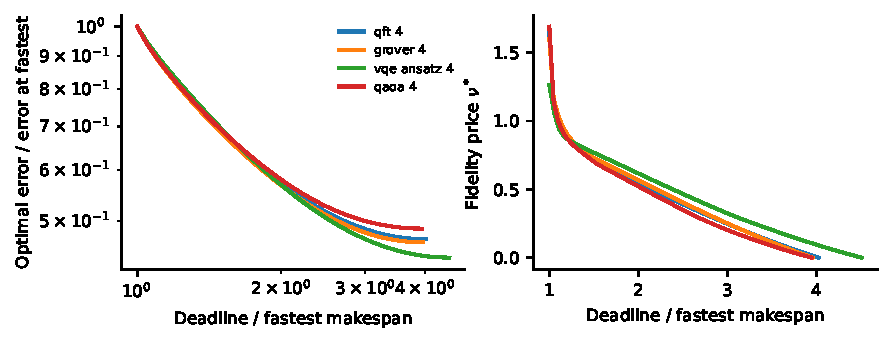
\includegraphics[width=\columnwidth]{figures/novelty_c7_frontier.pdf}
\caption{Latency--fidelity frontiers (left, log-log) and the dual fidelity price (right).}\label{fig:c7}
\end{figure}

\subsection{Pre-Registered Decoupling Test and Replication on IBM Heron}
Only delays and DD pulses are controllable on current IBM devices, so the hardware test targets Theorem~\ref{th:dd} with native durations fixed. The test has three stages.
\begin{itemize}
\item \textbf{Calibration H1} (\texttt{ibm\_marrakesh}, qubits 55, 54, 53; job \texttt{db54a1o4qg6s73c2v460}) measured CPMG decay for $n\in\{0,2,4,8\}$ and $w\in\{4,16,40,80\}\,\mu$s, and $T_1$. It revealed strong low-frequency, partly coherent detuning: one echo raises 16\,$\mu$s survival from 0.42 to about 0.90, and free precession revives after its first zero crossing. Before freezing, we therefore added a quasi-static term refocused by any balanced block and a readout offset. We capped pulse counts at the calibrated maximum of eight, because the uncapped fit would have inserted 2{,}358 pulses, and floored pulse error at the backend-reported $X$ error. Qubit 54 is poorly described by the model family.
\item \textbf{Test H2} (job \texttt{db54ep4vf2bc73cvcvbg}) fixed the model, the hash-verified circuits and the analysis before any data existed. It compared GP-DD with no DD, XX and XY4 on a GHZ-5 circuit with a 20\,$\mu$s ancilla wait, at a matched 24\,$\mu$s makespan on six qubits.
\item \textbf{Replication R1} (job \texttt{db54jfo4qg6s73c2ve5g}) repeated the identical circuits with four times the shots, under its own pre-registration and a pre-specified pooling rule.
\end{itemize}

\begin{table}[t]
\centering
\caption{Pre-registered decoupling test on IBM Heron (\texttt{ibm\_marrakesh}, qubits 55, 54, 53, 39, 33, 32; matched 24\,$\mu$s makespan): probability that all six qubits return to $|0\rangle$, with shot-only standard errors, and the primary difference with its shot-only 95\% interval. Pre-registered inverse-variance pooling: +2.18 pp, 95\% CI [+1.43, +2.92].}\label{tab:hw}
\footnotesize
\begin{adjustbox}{max width=\columnwidth}
\begin{tabular}{lcc}
\toprule
Policy & H2 (3$\times$2000 shots) & R1 (4$\times$6000 shots) \\
\midrule
GP-DD & 0.348 $\pm$ 0.006 & 0.326 $\pm$ 0.003 \\
GP-DD (cross-window, identical) & 0.345 $\pm$ 0.006 & 0.327 $\pm$ 0.003 \\
XY4-like & 0.338 $\pm$ 0.006 & 0.301 $\pm$ 0.003 \\
XX (Qiskit-like) & 0.321 $\pm$ 0.006 & 0.296 $\pm$ 0.003 \\
No DD & 0.290 $\pm$ 0.006 & 0.290 $\pm$ 0.003 \\
GP-DD $-$ best standard (pp) & +0.98 [-0.72, +2.68] & +2.46 [+1.63, +3.29] \\
\bottomrule
\end{tabular}
\end{adjustbox}
\end{table}


Table~\ref{tab:hw} reports the outcomes. In H2, GP-DD exceeded XY4 by $+0.98$ percentage points, with a shot-only interval $[-0.7,+2.7]$: not significant. In R1 the difference was $+2.46$ points $[+1.63,+3.29]$, with all blocks favouring GP-DD. The pre-registered pooled estimate is $+2.18$ points $[+1.43,+2.92]$. The model's predicted ranking of all five policies matched H2 exactly, and R1 up to a swap of two identical GP schedules. Its riskiest decision, leaving qubit 54 undecoupled, gave that qubit higher survival than XY4 in both runs (0.871 vs 0.846; 0.878 vs 0.858). Absolute fidelities drifted between runs while the two differences remained consistent. \paragraph{Control arms and a second qubit chain (H3).}
The comparison above leaves open whether GP-DD wins because of its per-qubit decisions or simply because it uses up to eight pulses per window where XY4 uses four. We therefore pre-registered a control study with four arms, each with 4 blocks $\times$ 6{,}000 shots:
\begin{itemize}
\item GP-DD;
\item a uniform CPMG-8 schedule placing eight pulses in every window where they fit, with nearly twice as many pulses as GP-DD;
\item GP-DD with the qubit the GP left undecoupled also protected;
\item XY4.
\end{itemize}
We ran it on chain A (job \texttt{db5549o4qg6s73c303kg}). We also ran it on a disjoint chain B (qubits 9, 8, 7, 6, 5, 4; calibration \texttt{db554vclf4us73c3i8ag}, test \texttt{db557cclf4us73c3ibeg}), chosen by lowest summed readout error after excluding chain A and its neighbours, with its own frozen model.

Table~\ref{tab:hw3} reports the outcomes. The primary comparison, GP-DD against uniform CPMG-8, is significant on both chains: $+1.69$ points $[+1.05,+2.32]$ on chain A and $+1.32$ points $[+0.46,+2.18]$ on chain B, with all blocks favouring GP-DD. The pre-registered pooled estimate is $+1.56$ points $[+1.05,+2.07]$. The advantage therefore comes from the allocation itself, not from pulse count: the GP schedule beats a schedule with nearly twice as many pulses. On chain A, leaving the poorly modelled qubit undecoupled was itself beneficial ($+0.71$ points $[+0.07,+1.35]$), and the predicted order of all four arms held.

On chain B, GP-DD tied XY4 ($+0.20$ points $[-0.67,+1.06]$), and the model's predicted order failed: it had predicted a large XY4 deficit. A plausible cause is that XY4 alternates $X$ and $Y$ pulses and is therefore robust to pulse errors, whereas our allocation inserts $X$-only CPMG blocks. Letting the GP choose robust sequence families as well as counts \cite{ezzell,tong2024,rahman2024} is a direct extension of Theorem~\ref{th:dd}, since the pulse-error coefficient $\epsilon_q$ simply becomes sequence-dependent.

Absolute fidelities on chain A drifted substantially between the morning runs and H3 (all arms near 0.13--0.16, against about 0.33 earlier), while the paired within-run comparisons remained consistent. Intervals are shot-only, and all runs used one device on one day. In total the hardware study used seven free-tier jobs and about two minutes of shot time.

\begin{table}[t]
\centering
\caption{Pre-registered control arms (H3) on \texttt{ibm\_marrakesh}, 4 blocks $\times$ 6000 shots per arm (Chain A: qubits 55, 54, 53, 39, 33, 32; Chain B: qubits 9, 8, 7, 6, 5, 4): all-qubit return probability with shot-only s.e., and paired differences with shot-only 95\% intervals. Pre-registered pooling of the primary over chains: +1.56 pp, 95\% CI [+1.05, +2.07].}\label{tab:hw3}
\footnotesize
\begin{adjustbox}{max width=\columnwidth}
\begin{tabular}{lcc}
\toprule
Arm / comparison & Chain A & Chain B \\
\midrule
GP-DD & 0.156 $\pm$ 0.002 & 0.371 $\pm$ 0.003 \\
GP-DD + protect GP-undecoupled qubit & 0.149 $\pm$ 0.002 & 0.369 $\pm$ 0.003 \\
Uniform CPMG-8 & 0.139 $\pm$ 0.002 & 0.358 $\pm$ 0.003 \\
XY4-like & 0.133 $\pm$ 0.002 & 0.369 $\pm$ 0.003 \\
GP-DD $-$ CPMG-8 (pp, primary) & +1.69 [+1.05, +2.32] & +1.32 [+0.46, +2.18] \\
GP-DD $-$ protect (pp) & +0.71 [+0.07, +1.35] & +0.23 [-0.63, +1.09] \\
GP-DD $-$ XY4 (pp) & +2.31 [+1.68, +2.94] & +0.20 [-0.67, +1.06] \\
Predicted order observed & yes & no \\
\bottomrule
\end{tabular}
\end{adjustbox}
\end{table}


\subsection{Multi-Scale Statistical Verification}
The following audits test implementation consistency against the declared model, rather than independent physical validity:
For twelve deterministic fixed-DAG instances with three, five, or eight gates, inverse powers one or two, and optional deadlines, we additionally bounded each computed GP objective with a supporting-hyperplane linear program solved independently by HiGHS. The maximum relative upper--lower gap was $1.10\times10^{-5}$. This bounds numerical suboptimality for the specified convex objective in these small instances; it cannot validate its empirical gate-error coefficients or establish a hardware gain.
\begin{enumerate}
\item \textbf{Dense Master Equations ($n=4$):} Comparison between analytical observable predictions and dense $16 \times 16$ density-matrix Lindblad simulation yielded a maximum deviation of $2.99 \times 10^{-15}$, confirming exact numerical agreement to machine precision.
\item \textbf{Forward Pauli-Frame Monte Carlo ($16{,}384$ shots):} Figure~\ref{fig:monte_carlo} displays forward Monte Carlo sampling deviations up to 32 qubits, verifying that empirical errors ($\le 0.0043$) remain strictly inside simultaneous Hoeffding confidence bounds ($\epsilon \approx 0.033\text{--}0.037$ at $\alpha = 0.001$).
\end{enumerate}

\begin{figure}[t]
\centering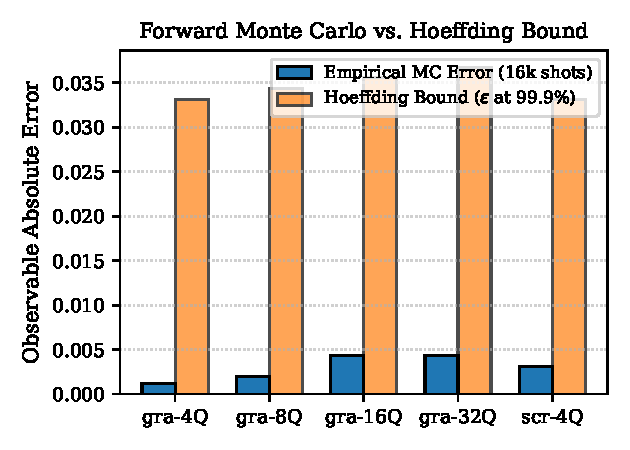
\includegraphics[width=0.92\columnwidth]{figures/observable_monte_carlo_validation.pdf}
\caption{Forward Pauli-frame Monte Carlo sampling validation ($16{,}384$ shots) across multi-qubit circuits. Empirical observable errors remain well below the simultaneous Hoeffding tolerance bounds ($\epsilon$ at 99.9\% confidence).}\label{fig:monte_carlo}
\end{figure}

\subsection{Interpretation of the Comparative Evidence}
The GP and ordinary convex formulations solve the same mathematical relaxation; their numerical agreement is a software and formulation check, not independent evidence that the physical model is accurate. The path-flow dual bracket bounds the optimum only for the declared fixed-DAG objective. The discrete-library transfer gap is sufficiently wide that it should not be read as a tight device-level performance certificate. Comparisons against the adapted slack heuristic are informative about modeled trade-offs, but unequal makespans confound unconstrained fidelity rankings. Accordingly, we treat matched-deadline results as the primary comparison and retain regressions. The 24 feasible large-circuit instances establish that the continuous solver can run at 128 qubits under attainable modeled targets; their makespan reductions (18\% or 31\%) are set by the assumed share $\alpha$. They do not resolve coefficient identification, idle noise, or hardware control feasibility.

\section{Discussion and Compiler Integration}

\subsection{End-to-End Compiler Pass Architecture}
We packaged the optimization engine as a native Qiskit \cite{qiskit2024} compilation pass (\texttt{ConvexDurationAllocationPass}), subclassing \texttt{AnalysisPass}. The pass operates directly on the transpiler's \texttt{DAGCircuit} representation through a streamlined pipeline:
\begin{enumerate}
\item \textbf{DAG Extraction:} Extracts the directed acyclic dependency graph $\mathcal{D}$, identifying causal scheduling precedence between successive gates on overlapping qubit supports without changing the gate order.
\item \textbf{Analytic Infeasibility Pre-Screening:} In $\mathcal{O}(\operatorname{nnz}(H))$ time, computes unconstrained gatewise noise minima $\tau_j^* = \operatorname{clip}(\sqrt{a_j/\gamma_j}, \ell_j, u_j)$ and evaluates $\max_k (\mu_k - \beta_k) \le 0$ with precomputed sensitivity matrix $H$. If violated, it records an analytic infeasibility diagnostic without invoking the numerical solver.
\item \textbf{Convex Duration Allocation:} Formulates the posynomial program with safety exposure $q\gamma_j$ and invokes Clarabel/CVXPY, yielding a numerical continuous-duration solution on feasible instances.
\item \textbf{Log-Grid Quantization:} Maps continuous allocations $\tau^*$ to an abstract geometric pulse library via upward ceiling quantization with box clamping $d_j^* = \min(u_j, \ell_j q^{\lceil \log_q (\tau_j^* / \ell_j) \rceil})$, with a conditional within-model feasibility bound.
\item \textbf{Property Set Annotation:} Annotates the pass manager's \texttt{property\_set} with duration vectors, modeled makespan, and any computed dual gap; the prototype does not synthesize executable pulses.
\end{enumerate}

\subsection{Algorithmic Routine and Constrained Dual Certification}
For observable-constrained duration allocation, let $w \in \mathbb{R}_+^K$ denote Lagrange multipliers for normalized observable constraints $\sum_j \frac{h_{kj}}{\beta_k}(a_j/\tau_j + q\gamma_j\tau_j) \le 1$. Grouping gate coefficients into $\tilde{A}_j(w) = a_j \sum_k \frac{w_k h_{kj}}{\beta_k}$ and $\tilde{C}_j(w) = q\gamma_j \sum_k \frac{w_k h_{kj}}{\beta_k}$, Lagrangian relaxation with dual DAG path pressure $\rho \in \frac{1}{\bar{M}}\operatorname{conv}(\mathcal{P})$ yields the constrained dual lower bound:
\begin{equation}\label{eq:constrained_dual}
D(w, \rho) = \sum_{j=1}^m \min_{\ell_j \le t \le u_j} \left[ \frac{\tilde{A}_j(w)}{t} + (\tilde{C}_j(w) + \rho_j)t \right] - \sum_{k=1}^K w_k.
\end{equation}
By weak duality, $D(w, \rho) \le M_{\mathrm{cont}}^*/\bar{M}$ for all dual-feasible $(w, \rho)$, where $M_{\mathrm{cont}}^* = \operatorname{LongestPath}(\mathcal{D}, \tau^*)$ is the optimal makespan of the continuous relaxation. The path-flow Frank--Wolfe routine ascends on $\rho$ to compute $D(w^*, \rho^*)$. The optimality gap certifies the numerical convergence bracket of this continuous solve:
\begin{equation}
\epsilon_{\mathrm{gap}} = \frac{M_{\mathrm{cont}}^*/\bar{M} - D(w^*, \rho^*)}{M_{\mathrm{cont}}^*/\bar{M}}.
\end{equation}
Subsequent discrete log-grid rounding yields discrete makespan $M_{\mathrm{disc}}^* = \operatorname{LongestPath}(\mathcal{D}, d^*)$, with guaranteed upper bound $M_{\mathrm{disc}}^* \le q M_{\mathrm{cont}}^*$. The complete routine is formalized in Algorithm~1.

\begin{table}[t]
\hrule\vspace{3pt}
\noindent\textbf{Algorithm 1:} Observable-Constrained Gate Duration Allocation\\[-0.5em]
\rule{\columnwidth}{0.4pt}\\[0.2em]
\footnotesize
\textbf{Input:} Circuit DAG $\mathcal{D}=(V, E)$, duration bounds $[\ell_j, u_j]$, noise rates $a_j, \gamma_j$, sensitivity matrix $H = (h_{kj}) \in \mathbb{R}^{K \times m}$, target observable fidelities $t_k^{\mathrm{target}}$, grid ratio $q > 1$, baseline makespan $\bar{M}$.\\
\textbf{Output:} Model-feasible discrete schedule $d^* \in \mathbb{R}^m$, discrete makespan $M_{\mathrm{disc}}^*$, continuous relaxation makespan $M_{\mathrm{cont}}^*$, relative optimality gap certificate $\epsilon_{\mathrm{gap}}$, or Infeasible diagnostic.
\begin{enumerate}
\itemsep 0.05em
\item Set $\beta_k \gets -\frac{1}{2} \ln t_k^{\mathrm{target}}$ for each target observable $k \in \{1, \dots, K\}$.
\item In $\mathcal{O}(m)$ time, compute gatewise unconstrained minimizers $\tau_j^{\mathrm{unc}} \gets \operatorname{clip}(\sqrt{a_j/\gamma_j}, \ell_j, u_j)$ and safety minimizers $\tau_j^{\mathrm{safe}} \gets \operatorname{clip}(\sqrt{a_j/(q\gamma_j)}, \ell_j, u_j)$.
\item In $\mathcal{O}(\operatorname{nnz}(H))$ time, compute lower-bound hazards:
$\mu \gets H(a/\tau^{\mathrm{unc}} + \gamma\tau^{\mathrm{unc}})$ and $\mu^{\mathrm{safe}} \gets H(a/\tau^{\mathrm{safe}} + q\gamma\tau^{\mathrm{safe}})$.
\item \textbf{if} $\max_k (\mu_k - \beta_k) > 0$ \textbf{then} \textbf{return} Infeasible (target unachievable under baseline noise).
\item \textbf{if} $\max_k (\mu_k^{\mathrm{safe}} - \beta_k) > 0$ \textbf{then} \textbf{return} Infeasible (safety margin $q$ uncertifiable).
\item Formulate convex posynomial program with safety exposure $\tilde{\gamma}_j \gets q\gamma_j$ (noting that off-critical gate durations are non-unique under makespan minimization per Remark~\ref{rem:uniqueness}):
\begin{equation*}
\begin{aligned}
\min_{\tau, f, M} \quad & M\\
\text{s.t.} \quad & \sum_{j} h_{kj} \left(\frac{a_j}{\tau_j} + q\gamma_j \tau_j\right) \le \beta_k, \quad \forall k,\\
& f_i + \tau_j \le f_j, \; \forall (i \to j) \in \mathcal{D}, \quad \tau_i \le f_i \le M,\\
& \ell_j \le \tau_j \le u_j, \quad \forall j.
\end{aligned}
\end{equation*}
\item Solve via Clarabel/CVXPY and check the returned primal constraint residual; reject a numerical result that exceeds the implemented feasibility tolerance. \textbf{if} solver status is infeasible \textbf{then} \textbf{return} Infeasible (no schedule satisfies precedence and bounds under safety margin $q$).
\item Retrieve continuous optimum $\tau^*$ and dual multipliers $w^* \ge 0$.
\item Compute continuous makespan $M_{\mathrm{cont}}^* \gets \operatorname{LongestPath}(\mathcal{D}, \tau^*)$.
\item Compute dual lower bound $D(w^*, \rho^*)$ via \eqref{eq:constrained_dual} and evaluate continuous gap:
\[ \epsilon_{\mathrm{gap}} \gets \frac{M_{\mathrm{cont}}^*/\bar{M} - D(w^*, \rho^*)}{M_{\mathrm{cont}}^*/\bar{M}}. \]
\item For each gate $j$, round upward with upper-bound box clamping:
\[ d_j^* \gets \min\left(u_j, \, \ell_j q^{\lceil \log_q (\tau_j^* / \ell_j) \rceil}\right). \]
\item Compute model-based discrete makespan $M_{\mathrm{disc}}^* \gets \operatorname{LongestPath}(\mathcal{D}, d^*)$.
\item \textbf{return} $d^*$, $M_{\mathrm{disc}}^*$, $M_{\mathrm{cont}}^*$, and primal--dual gap certificate $\epsilon_{\mathrm{gap}}$.
\end{enumerate}
\hrule
\end{table}

\subsection{Scope, Missing Baselines, and Physical Validation}
The geometric grid is an abstract library; it is not a measured set of alternate pulses on \emph{ibm\_torino}. A clock-aligned controller may require different rounding and an experimentally characterized noise response. The Qiskit implementation is an analysis pass that attaches duration results to a property set; it does not upload pulses or execute a modified schedule on hardware. The direct comparison uses Qiskit's published ASAP/ALAP and DD passes \cite{qiskit_sched}; it holds circuit and deadline fixed, but GP has hypothetical continuous-duration actions unavailable to those passes. Its rank reversal under static detuning limits rather than establishes a superiority claim.

The largest source of uncertainty for the target device is the unmeasured split between inverse-duration and duration-proportional hazards. The snapshot determines one nominal point per gate, so multiple duration-error curves interpolate it equally well. Varying $\alpha$ probes this model uncertainty but cannot estimate $\alpha$. The external measured single-qubit sweep shows that the assumed law can miss uncertainty-scale structure even where duration is varied experimentally; its coefficients cannot be transferred to IBM CZ gates. The Heron pilot varies \emph{idle} duration, not driven-gate duration; it cannot identify this split either. The first fixed-native-gate QPU check fails its prespecified nominal-model tolerance in every family; the second passes a six-family descriptive tolerance after a backend calibration update. Readout recalibration from a separate job did not improve the second check. Thus the fixed-gate results are calibration-sensitive and cannot establish model transfer across times, much less the duration dependence needed for GP deployment. An inverse-square candidate improves exploratory prediction error while preserving convexity, but remains inconsistent with reported measurement uncertainty and has no independent confirmation. The retrospective PCHIP decision audit improves choices in two families relative to the GP laws, but its larger-than-reported residuals and post hoc selection rule out a prospective accuracy claim. The GP proof for the evaluated circuit study still assumes isotropic post-gate Pauli noise and excludes schedule-dependent idle processes. The separate simulator probes anisotropic errors, idle $T_1/T_\phi$, and shot-static detuning during delays, but does not establish convexity for those additions. It omits detuning during driven gates, coherent crosstalk, leakage, and pulse-shape dependence. Dense Lindblad and Monte Carlo agreement only establish that separate implementations evaluate their shared assumed model consistently.

The native X experiment establishes that two supported gate durations can yield different physical returns under a matched schedule, and that a training-selected slow implementation can outperform equal-duration delayed-X and standard two-X DD controls on one held-out X-basis task. It does not show that the proposed inverse-plus-linear law chose the gate, that a GP solver improved hardware output, or that the ranking persists across bases: the Z-basis control reverses it. A gate-dependent, observable-aware model that accounts for driven evolution and coherent idle effects must be specified and fitted on one set of durations/circuits, then prospectively tested on independent choices and circuits. The existing two-point X library cannot identify a robust duration-response curve or test a continuous optimum. The pre-registered decoupling test of Section~IX addresses part of this gap. There, a GP-selected schedule was executed on hardware, its predicted policy ranking held, and it beat XY4 in a replicated comparison. Because current devices do not expose gate-duration control, that test exercises only the idle and DD decisions of Theorem~\ref{th:dd}; the duration-allocation results remain simulation-only. Wider hardware-compatible pulse libraries, other qubit chains and devices, and repeated calibration cycles are necessary before asserting general hardware benefit.

\section{Conclusion}
Geometric programming is the native structure of fidelity-driven quantum resource allocation. For a fixed circuit DAG and declared inverse-plus-linear noise model, gate-duration allocation has an exact convex representation and an inspectable path-flow lower bound. The same convex structure accommodates a declared positive inverse-power model. Under post-gate isotropic Pauli noise on Clifford circuits, stabilizer-expectation targets produce convex constraints and conditional safe rounding for the evaluated law. The model-attainable study shows feasible continuous solves through 128 qubits, while the original strict-target study mainly demonstrates fast analytic rejection. Experimental duration sweeps reveal sizeable departures from the evaluated two-parameter law; an exploratory inverse-square variant reduces prediction error but does not explain reported uncertainty. A retrospective empirical finite-library predictor improves selected measured durations in two pulse families without validating the GP error law. The direct local GP-versus-Qiskit comparison shows only small modeled Markovian gains and a substantial regression against DD under shot-static detuning. The Heron idle pilot (Appendix~\ref{app:idle_pilot}) observes idle-time dependence and coherent dephasing; two fixed-native-gate checks (Appendix~\ref{app:model_checks}) demonstrate calibration-sensitive discrepancies. A further training-selected, held-out native-X experiment demonstrates an X-basis return improvement on one qubit, with a Z-basis reversal that, by Proposition~\ref{prop:iso}, falsifies isotropic noise models.

Beyond gate durations, the same log-posynomial structure yields exact joint allocation of timing and dynamical decoupling, closed-form runtime optima for mitigated estimation, certified robustness with baseline dominance, anisotropic and state-aware constraints, and sharp hardness and approximation statements. Simulations characterize where these help: duration control and decoupling gain on average, while low-frequency noise shared across idle windows remains the main failure mode. In a pre-registered and replicated test on IBM Heron, a GP-selected decoupling schedule beat the best standard sequence by 2.2 percentage points, and the model predicted the ranking of five policies in advance. Pre-registered controls on two disjoint qubit chains attribute the gain to the allocation itself: GP-DD beats a uniform schedule with nearly twice as many pulses by 1.6 points (pooled interval 1.0--2.1). Against XY4 the advantage is chain-dependent, which motivates letting the GP choose pulse-error-robust sequence families. Tests across devices and days are the next step.

\appendices

\section{Full Proofs of the Framework Results}\label{app:proofs}
Throughout, $y=\log\tau$ componentwise, $\mathcal P$ is the set of source--sink path incidence vectors of the fixed DAG, and $M(\tau)=\max_{p\in\mathcal P}p^\top\tau$.

\subsection{Proof of Theorem~\ref{th:catalogue} (Catalogue)}
\emph{(i)} For a single Pauli $P$ with rate $\lambda$, the Lindblad generator $\mathcal L(\rho)=\lambda(P\rho P-\rho)$ has adjoint $\mathcal L^\dagger(O)=\lambda(POP-O)$. For a Pauli observable $O$, $POP=-O$ if $\{P,O\}=0$ and $POP=O$ otherwise. Hence $e^{t\mathcal L^\dagger}(O)=e^{-2\lambda t}O$ or $O$. Generators for different Paulis commute, because each maps every Pauli to a multiple of itself, so the channel of gate $j$ multiplies $O$ by $\exp(-2\sum_{P\in\mathcal A(O)}\lambda_{jP})$. An ideal Clifford maps a Pauli to a Pauli, up to sign, and preserves this structure. Propagating $S_k$ backward through the circuit, the factor at gate $j$ is fixed by the propagated operator $S_k(t_j)$, and multiplying the factors gives the formula. Since $\langle S_k\rangle_{\mathrm{ideal}}=1$, the constraint $\langle S_k\rangle\ge t_k$ is equivalent to $\sum_j\sum_{P\in\mathcal A_{kj}}\lambda_{jP}\le-\tfrac12\ln t_k$. Its left side is a sum of posynomials with nonnegative weights, hence a posynomial.

\emph{(ii)} The single-Pauli channel $\mathcal E(\rho)=(1-q)\rho+qP\rho P$ with $q=(1-e^{-2\lambda})/2$ acts on Paulis as identity or multiplication by $1-2q=e^{-2\lambda}$. The map $\mathcal E^{-1}(\rho)=\alpha\rho-\beta P\rho P$ with $\alpha=(e^{2\lambda}+1)/2$ and $\beta=(e^{2\lambda}-1)/2$ satisfies $\alpha+\beta\cdot(\pm1)\in\{1,e^{2\lambda}\}$ on the corresponding Paulis, and so inverts $\mathcal E$. Sampling the identity with probability $\alpha/\gamma_P$ and $P$ with probability $\beta/\gamma_P$, with sign $-1$, where $\gamma_P=\alpha+\beta=e^{2\lambda}$, gives an unbiased estimator after multiplication by $\gamma_P$. Independent insertions compose, so the total weight is $\gamma=\prod\gamma_P=\exp(2\sum\lambda_{jP})$. Each shot returns $\pm\gamma$, so $\mathbb E[X^2]=\gamma^2$ and $\operatorname{Var}X=\gamma^2-\langle O\rangle^2$.

\emph{(iii)} A posynomial $\sum_k c_k\prod_j x_j^{\alpha_{kj}}$ with $c_k>0$ becomes $\sum_kc_ke^{\alpha_k^\top y}$, a nonnegative combination of exponentials of affine functions and therefore convex in $y$. Hence $\log\gamma=2\sum\lambda_{jP}(e^y)$ is convex, and $\log(\gamma^2/s)=2\log\gamma-\log s$ is convex jointly in $(y,\log s)$.

\subsection{Proof of Theorem~\ref{th:dd} and Corollaries~\ref{cor:n}--\ref{cor:threshold}}
For $\beta\ge0$, $\phi(x)=x^{1+\beta}$ is convex on $x\ge0$. Its perspective $g(w,t)=t\,\phi(w/t)=w^{1+\beta}t^{-\beta}$ is jointly convex on $\{w\ge0,t>0\}$ \cite[\S3.2.6]{boydbook}. Each window width $w_k$ is an affine function of the start times, the durations and $M$, and $t_k=n_k+1$ is affine in $n_k$. The composition of a convex function with an affine map is convex, so every term $c_qw_k^{1+\beta_q}(n_k+1)^{-\beta_q}$ is convex. The terms $\eta_qw_k$, $\epsilon_qn_k$ and $g_j\tau_j$ are linear, $a_j/\tau_j$ is convex on $\tau_j>0$, and all constraints are linear. The feasible set of integer pulse counts is contained in the real relaxation, so the relaxed optimum is a lower bound. For Corollary~\ref{cor:n}, with $w$ fixed, $f(n)=cw^{1+\beta}(n+1)^{-\beta}+\epsilon n$ is convex in $n$, and $f'(n)=-\beta cw^{1+\beta}(n+1)^{-\beta-1}+\epsilon=0$ gives the stated $n^\star$. Projecting onto $[0,w/\tau_\pi]$ preserves optimality for a convex function of one variable, and the best even integer is one of the two even integers bracketing $n^\star$. For Corollary~\ref{cor:threshold}, under the stated one-for-one coupling the objective restricted to $\tau_j$ is $a_j/\tau_j+(g_j-\bar\eta_j)\tau_j+\mathrm{const}$. If $g_j>\bar\eta_j$ its unconstrained minimizer is $\sqrt{a_j/(g_j-\bar\eta_j)}$, and clipping gives the constrained one. Otherwise the function is decreasing in $\tau_j$, so the largest feasible duration is optimal. The strictly convex term $a_j/\tau_j$ fixes $\tau_j$ uniquely whenever $a_j>0$, which removes the non-uniqueness noted in Remark~\ref{rem:uniqueness}.

\subsection{Proof of Proposition~\ref{prop:state}}
\emph{(i)} A gate acting on qubits other than $q$ is a unitary $V\otimes I_q$, and the partial trace over those qubits is invariant under such a unitary. Hence the reduced state of $q$, and its excited population $p_1$, is constant between consecutive gates on $q$. Under an even CPMG block with pulses at $w(2i+1)/(2n)$, the qubit spends segments of length $w/(2n)$, $w/n$, \dots, $w/(2n)$ alternately in the original and flipped computational populations. The unflipped total is $w/(2n)+(n/2-1)w/n+w/(2n)=w/2$, so the time-averaged excited population is exactly $1/2$. The weights $p_1\ge0$ and $1/2$ multiply terms linear in $w$, so convexity is preserved. Since $\min(p_1,1/2)$ is at most the weight of every integer choice, using it in the relaxation keeps the relaxed value a lower bound.

\emph{(ii)} For fixed widths $w_k\ge0$, $U(z)=\sum_kw_k(1-z_k)$ is affine and nonnegative on $[0,1]^K$. The maps $x\mapsto x^{1+\beta}$ and $x\mapsto x^2$ are convex and nondecreasing on $x\ge0$, so their compositions with $U$ are convex. The remaining terms are linear in $z$, and terms for different qubits involve disjoint variables, so the objective separates. Each qubit's binary problem has $2^{K_q}$ assignments and is solved exactly by enumeration.

\subsection{Proof of Theorem~\ref{th:runtime}}
Write $L(y)=\log T(e^y)=4\Lambda(e^y)+\log(M(e^y)+t_{\rm rep})-2\log\epsilon$. Here $\Lambda(e^y)=\sum_j(a_je^{-y_j}+g_je^{y_j})$ is convex. For each path $p$, $\log(\sum_{j\in p}e^{y_j}+t_{\rm rep})$ is a log-sum-exp of affine functions of $y$ (with the constant term written as $e^{\log t_{\rm rep}}$), hence convex. $\log(M+t_{\rm rep})$ is the maximum over paths of these functions, because $\log$ is increasing, and is therefore convex. By Danskin's theorem, $\partial_\tau M(\tau)=\operatorname{conv}\{p:p^\top\tau=M(\tau)\}$. At an optimum with $\tau_j$ in the interior of $[\ell_j,u_j]$, the first-order condition in $\tau_j$ reads $4(-a_j/\tau_j^2+g_j)+p_j/(M+t_{\rm rep})=0$ for some $p\in\partial M$. Solving for $\tau_j$ gives the formula. Each $p_j\in[0,1]$, and $p_j=0$ unless gate $j$ lies on a critical path. As $t_{\rm rep}\to\infty$ with $p_j$ bounded, $p_j/(4(M+t_{\rm rep}))\to0$, so $\tau_j^\star\to\sqrt{a_j/g_j}$.

\subsection{Proofs of Theorems~\ref{th:coverage}--\ref{th:dominance}}
\emph{Worst case.} The error is linear in the parameters: $E_\theta(\tau)=\sum_g\theta_g^\top v_g(\tau)$. Over the ellipsoid $\{\theta:\sum_g(\theta_g-\hat\theta_g)^\top\Sigma_g^{-1}(\theta_g-\hat\theta_g)\le\kappa^2\}$, write $\theta_g=\hat\theta_g+\Sigma_g^{1/2}u_g$ with $\sum_g\|u_g\|^2\le\kappa^2$. By Cauchy--Schwarz, $\sup\sum_gu_g^\top\Sigma_g^{1/2}v_g=\kappa(\sum_gv_g^\top\Sigma_gv_g)^{1/2}$.

\emph{Diagonal bound.} For $2\times2$ positive semidefinite $\Sigma$, $2\operatorname{diag}(\Sigma)-\Sigma=\begin{pmatrix}\sigma_{11}&-\sigma_{12}\\-\sigma_{12}&\sigma_{22}\end{pmatrix}$ has nonnegative diagonal and determinant $\sigma_{11}\sigma_{22}-\sigma_{12}^2\ge0$, so it is positive semidefinite. When $\Sigma$ is diagonal the factor 2 is unnecessary.

\emph{Clipping.} Since $v_g\ge0$, replacing $\hat\theta$ by $\hat\theta^+=\max(\hat\theta,0)$ shifts the ellipsoid upward, which can only increase the supremum, so $C(\tau)$ remains an upper bound.

\emph{GP form.} Each $v_{g,i}$ is a posynomial, so is its square, and so is the weighted sum $Q(\tau)$. Introducing $r>0$ with $Q(\tau)/r^2\le1$, a posynomial constraint, makes $\kappa r$ an epigraph variable for $\kappa\sqrt{Q}$, and the objective $E_{\hat\theta^+}+\kappa r$ is a posynomial.

\emph{Coverage.} If $\hat\theta_g\sim\mathcal N(\theta_g,\Sigma_g)$ independently, then $\sum_g(\hat\theta_g-\theta_g)^\top\Sigma_g^{-1}(\hat\theta_g-\theta_g)\sim\chi^2_{2G}$. With $\kappa^2$ its $(1-\delta)$ quantile, the true $\theta$ lies in the ellipsoid with probability $1-\delta$. On that event the bound holds for every $\tau$ simultaneously, including the data-dependent optimizer.

\emph{Dominance.} The baseline $\tau^0$ satisfies every added constraint with equality, so the problem stays feasible. For $E=\sum_s\mu_sE_s$ with $\mu$ in the simplex, linearity in the coefficients gives $E(\hat\tau)=\sum_s\mu_sE_s(\hat\tau)\le\sum_s\mu_sE_s(\tau^0)=E(\tau^0)$. Each $E_s$ is a posynomial, so each added constraint $E_s(\tau)/E_s(\tau^0)\le1$ is a posynomial constraint.

\subsection{Proof of Proposition~\ref{prop:iso}}
Identify $k$-qubit Paulis, up to phase, with $\mathbb F_2^{2k}$, and let $\omega$ be the symplectic form. For a nonzero $r$, the map $x\mapsto\omega(x,r)$ is a nonzero linear functional, so its kernel has exactly $4^k/2$ elements, and exactly $2\cdot4^{k-1}$ Paulis anticommute with $r$. The identity is in the kernel, so all anticommuting Paulis are non-identity. Under an isotropic channel every non-identity Pauli has rate $\lambda_j/(4^k-1)$. The decay factor of gate $j$ on any observable whose back-propagated restriction to $\operatorname{supp}(j)$ is non-identity is therefore $\exp(-2\lambda_j\cdot2\cdot4^{k-1}/(4^k-1))$, independent of which Pauli the restriction is. Two observables whose back-propagated supports meet the same set of gates therefore decay identically. For single-qubit observables on one wire this holds for $X$, $Y$ and $Z$ alike, so every schedule ranking by single-qubit survival is the same in all three bases.

\subsection{Proof of Theorem~\ref{th:hard} (Hardness)}
The deadline discrete time--cost trade-off problem (DTCTP) is as follows. Given an activity-on-node DAG $G=(V,A)$, for each activity $v$ a finite set of modes $(t_{v,i},c_{v,i})$, a deadline $T$ and a budget $C$, decide whether some mode choice has longest path at most $T$ and total cost at most $C$. It is strongly NP-hard \cite{de1997}.

\emph{Construction.} Given an instance, build a circuit with one qubit $q_e$ for each arc $e=(u,v)\in A$, plus one private qubit per activity so that every gate acts on at least one qubit. Gate $g_v$ acts on its private qubit and on every $q_e$ with $e$ incident to $v$, and gates are ordered by any topological order of $G$. Qubit $q_e$ is touched only by $g_u$ and $g_v$, so the circuit's dependency DAG has exactly the arcs $A$. The library of $g_v$ is $\{(t_{v,i},c_{v,i})\}$, read as (duration, characterized error), the deadline is $T$, and the question is whether total error can be at most $C$. Feasible schedules and their makespans and errors correspond one-to-one with mode choices and their durations and costs, and the construction is polynomial with numbers unchanged, so strong NP-hardness transfers. Gate arity equals vertex degree plus one, so the reduction needs gates of unbounded arity, as stated.

\subsection{Proof of Theorem~\ref{th:bicriteria} (Bicriteria Rounding)}
Let $\tau^c$ minimize $E_q(\tau)=\sum_j(a_j/\tau_j+qg_j\tau_j)$ subject to $M(\tau)\le D$ and $\ell\le\tau\le u$. For $\tau^c_j\in[\ell_j,u_j]$, let $\tau^r_j=\min(u_j,\ell_jq^{\lceil\log_q(\tau^c_j/\ell_j)\rceil})$. Then $\tau^c_j\le\tau^r_j\le q\tau^c_j$: the grid point is the smallest one at least $\tau^c_j$, consecutive grid points differ by a factor $q$, and clamping at $u_j\ge\tau^c_j$ keeps the lower bound. Path sums are monotone and positively homogeneous, so $M(\tau^r)\le M(q\tau^c)=qM(\tau^c)\le qD$. Next, $E(\tau^r)=\sum_j(a_j/\tau^r_j+g_j\tau^r_j)\le\sum_j(a_j/\tau^c_j+qg_j\tau^c_j)=E_q(\tau^c)$. For any feasible $\tau$, $E_q(\tau)\le qE(\tau)$ because $q\ge1$, so $E_q(\tau^c)\le q\min E=q\,\mathrm{OPT}_{\mathrm{cont}}(D)$. Every schedule built from a library $L\subset[\ell,u]$ that meets $D$ is feasible for the continuous problem, so $\mathrm{OPT}_{\mathrm{cont}}(D)\le\mathrm{OPT}_L(D)$.

\subsection{Proof of Proposition~\ref{prop:frontier} (Frontier)}
In the variables $y=\log\tau$ the problem is $\min f_0(y)$ subject to the convex constraints $y\in[\log\ell,\log u]$ and $g(y)\le d$, with $f_0=\log E(e^y)$ (log of a posynomial, convex) and $g=\log M(e^y)$ (convex, as above). The optimal value $F(d)=\inf\{f_0(y):g(y)\le d,\ y\in[\log\ell,\log u]\}$ is a convex function of $d$, since for $d_\theta=\theta d_1+(1-\theta)d_2$ the convex combination of feasible points is feasible and $f_0$ is convex. Slater's condition holds for $d$ above the minimum attainable $\log M$, so strong duality holds, and $-\nu^\star(d)\in\partial F(d)$ for the optimal multiplier $\nu^\star$ of $g(y)\le d$ \cite[\S5.6]{boydbook}. Where $F$ is differentiable, $F'(d)=-\nu^\star(d)$. Since $F(d)=\log E^\star(e^d)$, the stated identity follows.

\section{Exploratory Heron Idle-Noise Pilot}\label{app:idle_pilot}
We executed a small, separate timing pilot on \texttt{ibm\_marrakesh} through the free Open instance (job \texttt{db4ll9o4qg6s73c2buj0}). Four one-qubit circuits on physical qubit 0 were interleaved in two shuffled blocks, with 2,048 shots per circuit. Each prepared and measured an $X$-basis state with two logical Hadamards. The three Ramsey circuits inserted a 1, 20, or 80~$\mu$s idle delay; the fourth inserted two 40~$\mu$s delays separated by $X$, followed by a second $X$ before the final Hadamard, preserving the ideal operation. Qiskit transpilation at optimization level zero retained all requested delays. The backend calibration snapshot immediately preceding the job reported $T_1=298.5~\mu$s and $T_2=40.4~\mu$s for that qubit.

Table~\ref{tab:hardware_idle} gives the raw outcome fractions. Both blocks showed a higher zero frequency with the echo sequence than with the 80-$\mu$s Ramsey sequence; the blockwise differences were 0.1021 and 0.1201. This is exploratory evidence that idle dynamics and control placement matter on the target architecture. Importantly, the 80~$\mu$s Ramsey outcome $P(0) = 0.4753$ sits approximately $3\sigma$ below $0.5$ (the completely mixed state), pointing to coherent phase accumulation and detuning rather than pure exponential $T_2$ dephasing. It is not a matched gate-count comparison, does not isolate a decay constant from coherent detuning and readout effects, and does not test a GP-selected gate duration. The job consumed 7~s of the free QPU allowance.

\begin{table}[t]
\centering\caption{Exploratory \emph{ibm\_marrakesh} idle-noise pilot on physical qubit 0: two blocks per condition, 2,048 shots per block. $P(0)$ is an observed frequency, not circuit fidelity.}\label{tab:hardware_idle}
\begin{tabular}{lcc}\hline
Circuit & Zero counts/shots & $P(0)$\\\hline
Ramsey, 1~$\mu$s & 4025/4096 & 0.9827\\
Ramsey, 20~$\mu$s & 2655/4096 & 0.6482\\
Ramsey, 80~$\mu$s & 1947/4096 & 0.4753\\
Echo, 80~$\mu$s & 2402/4096 & 0.5864\\\hline
\end{tabular}
\end{table}

\section{Prespecified Heron Native-Gate Model Checks and Relative Error Analysis}\label{app:model_checks}
We tested whether the declared independent post-gate isotropic Pauli model, anchored to the backend's reported nominal gate errors and independent readout assignment errors, predicts outcomes for fixed native gates. Before submission, we saved a calibration snapshot and predicted distributions for four small Clifford circuit families, compiled to physical qubits 0--2 on \texttt{ibm\_marrakesh}. Three shuffled blocks each contained one instance of every family, with 2,048 shots per instance (job \texttt{db4nov04qg6s73c2e8d0}). The prespecified events were return to \texttt{0}, Bell parity \texttt{00}/\texttt{11}, Bell return to \texttt{00}, and GHZ parity \texttt{000}/\texttt{111}.

\begin{table}[t]
\centering\small\setlength{\tabcolsep}{2.5pt}\caption{Prespecified nominal native-gate model check on \emph{ibm\_marrakesh}; each family has three blocks of 2,048 shots. Residual is observed minus pre-job predicted event probability.}\label{tab:hardware_model}
\begin{tabular}{lcccc}\hline
Family & Successes/6144 & Predicted & Residual & Rel. Error\\\hline
Single return & 6119 & 0.9685 & +0.0274 & +2.8\%\\
Bell parity & 6065 & 0.9619 & +0.0253 & +2.6\%\\
Bell return & 6000 & 0.9512 & +0.0254 & +2.7\%\\
GHZ parity & 5984 & 0.9201 & +0.0538 & +5.8\%\\\hline
\end{tabular}
\end{table}

All four discrepancies exceed the prespecified absolute tolerance of 0.02. Crucially, the descriptive absolute tolerance of 0.02 is loose relative to target device gate error rates ($0.3\%\text{--}4.8\%$). In relative error metrics, the model underpredicts hardware success by $+2.6\%$ to $+5.8\%$. The pre-job snapshot's qubit-0 probability of reporting 1 after preparing 0 was 0.03027, while the return circuit produced only 25 ones in 6,144 shots. This suggests calibration drift or unmodeled state-preparation fidelity.

We then froze a separate diagnostic before collecting new data: 18 readout-calibration circuits ($|0\rangle$ and $X|0\rangle$ on each of qubits 0--2, in three randomized blocks) and 18 held-out target circuits (six families in three randomized blocks), each at 2,048 shots. The calibration job \texttt{db4o3784qg6s73c2ekqg} completed before a SHA-256 lock of both the new backend-snapshot and empirically readout-adjusted predictions; only then was target job \texttt{db4o3bo4qg6s73c2ekvg} submitted.

\begin{table}[t]
\centering\small\setlength{\tabcolsep}{2.5pt}\caption{Second, held-out fixed-native-gate check on \emph{ibm\_marrakesh}: three 2,048-shot blocks per family. Entries are target-event probabilities; calibrated predictions change only measured operational readout parameters.}\label{tab:hardware_readout}
\begin{tabular}{lcccc}\hline
Family & Observed & Snapshot & Calibrated & Rel. Error\\\hline
Single return & 0.9937 & 0.9948 & 0.9951 & -0.1\%\\
Single-one return & 0.9919 & 0.9917 & 0.9924 & +0.0\%\\
Bell parity & 0.9849 & 0.9871 & 0.9872 & -0.2\%\\
Bell return & 0.9740 & 0.9825 & 0.9851 & -0.9\%\\
GHZ parity & 0.9723 & 0.9728 & 0.9755 & -0.1\%\\
GHZ return & 0.9587 & 0.9632 & 0.9686 & -0.5\%\\\hline
\end{tabular}
\end{table}

While all six readout-adjusted event residuals were below the absolute 0.02 tolerance, the model now slightly overpredicts hardware success (relative errors ranging from $-0.1\%$ to $-0.9\%$), and the raw snapshot prediction was more accurate overall than the empirical readout correction (mean absolute error 0.00286 versus 0.00476). The new backend calibration, time-stamped 02:47 local time, reported much smaller qubit-0 and qubit-2 readout errors than the earlier 02:28 snapshot (e.g., $P(1|0)$ on qubit 0 fell from 0.03027 to 0.00391). This sign reversal across consecutive jobs highlights temporal calibration drift. These fixed-gate observations neither validate the duration-error law nor demonstrate a GP schedule advantage.

\section*{Statements and Declarations}
\noindent\textbf{Funding.} No funds, grants, or other support were received for this study.\par
\noindent\textbf{Competing interests.} The author declares no relevant financial or non-financial competing interests.\par
\noindent\textbf{Data and code availability.} The source, frozen protocols, raw QPU counts and QPY circuits, analysis scripts, benchmark outputs, and manuscript source are available at \url{https://github.com/Youssef-Ahmed38/quantum-gp-circuit-optimization} and in the accompanying supplementary archive (Online Resource 1).\par

\begin{thebibliography}{40}
\bibitem{kelley} J. E. Kelley, ``Critical-path planning and scheduling: Mathematical basis,'' \emph{Operations Research}, vol. 9, no. 3, pp. 296--320, 1961.
\bibitem{fulkerson} D. R. Fulkerson, ``A network flow computation for project cost curves,'' \emph{Management Science}, vol. 7, no. 2, pp. 167--178, 1961.
\bibitem{boydgp} S. Boyd, S.-J. Kim, L. Vandenberghe, and A. Hassibi, ``A tutorial on geometric programming,'' \emph{Optimization and Engineering}, vol. 8, no. 1, pp. 67--127, 2007.
\bibitem{boyddigital} S. Boyd, S.-J. Kim, D. Patil, and M. Horowitz, ``Digital circuit optimization via geometric programming,'' \emph{Operations Research}, vol. 53, no. 6, pp. 899--932, 2005.
\bibitem{lussi} E. W. Lussi, R. de Santiago, and E. I. Duzzioni, ``Time-optimization framework for the implementation of robust low-latency quantum circuits,'' \emph{Physical Review Applied}, vol. 23, Art. no. 044036, 2025, doi: 10.1103/PhysRevApplied.23.044036.
\bibitem{ahuja} R. K. Ahuja, D. S. Hochbaum, and J. B. Orlin, ``Solving the convex cost integer dual network flow problem,'' \emph{Management Science}, vol. 49, no. 7, pp. 950--964, 2003.
\bibitem{dalibard} J. Dalibard, Y. Castin, and K. M\o lmer, ``Wave-function approach to dissipative processes in quantum optics,'' \emph{Physical Review Letters}, vol. 68, pp. 580--583, 1992.
\bibitem{jaggi} M. Jaggi, ``Revisiting Frank-Wolfe: Projection-free sparse convex optimization,'' in \emph{Proceedings of Machine Learning Research}, vol. 28, no. 1, pp. 427--435, 2013.
\bibitem{watrous} J. Watrous, ``Simpler semidefinite programs for completely bounded norms,'' \emph{Chicago Journal of Theoretical Computer Science}, Art. no. 8, 2013.
\bibitem{hung} S.-H. Hung, K. Hietala, S. Zhu, M. Ying, M. Hicks, and X. Wu, ``Quantitative robustness analysis of quantum programs,'' \emph{Proceedings of the ACM on Programming Languages}, vol. 3, POPL, Art. no. 31, 2019.
\bibitem{kosut} R. L. Kosut, M. D. Grace, and C. Brif, ``Robust control of quantum gates via sequential convex programming,'' \emph{Physical Review A}, vol. 88, Art. no. 052326, 2013.
\bibitem{murali_noise} P. Murali, J. M. Baker, A. Javadi-Abhari, F. T. Chong, and M. Martonosi, ``Noise-adaptive compiler mappings for noisy intermediate-scale quantum computers,'' in \emph{Proc. ASPLOS}, pp. 1015--1029, 2019.
\bibitem{murali_crosstalk} P. Murali, D. C. McKay, M. Martonosi, and A. Javadi-Abhari, ``Software mitigation of crosstalk on noisy intermediate-scale quantum computers,'' in \emph{Proc. ASPLOS}, pp. 1001--1016, 2020.
\bibitem{earnest} N. Earnest et al., ``Pulse-efficient circuit transpilation for quantum applications on cross-resonance-based architectures,'' \emph{Physical Review Research}, vol. 3, no. 4, Art. no. 043088, 2021, doi: 10.1103/PhysRevResearch.3.043088.
\bibitem{vandenberg} E. van den Berg, Z. K. Minev, A. Kandala, and K. Temme, ``Probabilistic error cancellation with sparse Pauli--Lindblad models on noisy quantum processors,'' \emph{Nature Physics}, vol. 19, pp. 1116--1121, 2023, doi: 10.1038/s41567-023-02042-2.
\bibitem{aigner} P. Aigner, J. Matti, M. F. Mor-Ruiz, J. Walln\"ofer, and W. D\"ur, ``Analytical and compressed simulation of noisy stabilizer circuits,'' \emph{arXiv preprint arXiv:2604.22588}, 2026.
\bibitem{qiskit_sched} IBM Quantum, ``Create a pass manager for dynamical decoupling,'' \emph{IBM Quantum Documentation}. [Online]. Available: \url{https://docs.quantum.ibm.com/guides/dynamical-decoupling-pass-manager}. Accessed: Oct. 9, 2026.
\bibitem{viola_dd} L. Viola, E. Knill, and S. Lloyd, ``Dynamical decoupling of open quantum systems,'' \emph{Physical Review Letters}, vol. 82, no. 12, pp. 2417--2421, 1999, doi: 10.1103/PhysRevLett.82.2417.
\bibitem{hyyppa_data} E. Hyypp\"a \emph{et al.}, ``Data for Reducing leakage of single-qubit gates for superconducting quantum processors using analytical control pulse envelopes,'' Zenodo, 2024, doi: 10.5281/zenodo.13808824.
\bibitem{uhrig} G. S. Uhrig, ``Keeping a quantum bit alive by optimized $\pi$-pulse sequences,'' \emph{Physical Review Letters}, vol. 98, Art. no. 100504, 2007, doi: 10.1103/PhysRevLett.98.100504.
\bibitem{cywinski} {\L}. Cywi\'nski, R. M. Lutchyn, C. P. Nave, and S. Das Sarma, ``How to enhance dephasing time in superconducting qubits,'' \emph{Physical Review B}, vol. 77, Art. no. 174509, 2008, doi: 10.1103/PhysRevB.77.174509.
\bibitem{biercuk} M. J. Biercuk, A. C. Doherty, and H. Uys, ``Dynamical decoupling sequence construction as a filter-design problem,'' \emph{Journal of Physics B: Atomic, Molecular and Optical Physics}, vol. 44, Art. no. 154002, 2011.
\bibitem{adapt} P. Das, S. Tannu, S. Dangwal, and M. Qureshi, ``ADAPT: Mitigating idling errors in qubits via adaptive dynamical decoupling,'' in \emph{Proc. 54th IEEE/ACM International Symposium on Microarchitecture (MICRO)}, 2021.
\bibitem{vaqem} G. S. Ravi, K. N. Smith, P. Gokhale, A. Mari, N. Earnest, A. Javadi-Abhari, and F. T. Chong, ``VAQEM: A variational approach to quantum error mitigation,'' in \emph{Proc. IEEE International Symposium on High-Performance Computer Architecture (HPCA)}, 2022, doi: 10.1109/HPCA53966.2022.00029.
\bibitem{ezzell} N. Ezzell, B. Pokharel, L. Tewala, G. Quiroz, and D. A. Lidar, ``Dynamical decoupling for superconducting qubits: A performance survey,'' \emph{Physical Review Applied}, vol. 20, Art. no. 064027, 2023, doi: 10.1103/PhysRevApplied.20.064027.
\bibitem{temme} K. Temme, S. Bravyi, and J. M. Gambetta, ``Error mitigation for short-depth quantum circuits,'' \emph{Physical Review Letters}, vol. 119, Art. no. 180509, 2017, doi: 10.1103/PhysRevLett.119.180509.
\bibitem{de1997} P. De, E. J. Dunne, J. B. Ghosh, and C. E. Wells, ``Complexity of the discrete time-cost tradeoff problem for project networks,'' \emph{Operations Research}, vol. 45, no. 2, pp. 302--306, 1997, doi: 10.1287/opre.45.2.302.
\bibitem{boydbook} S. Boyd and L. Vandenberghe, \emph{Convex Optimization}. Cambridge, U.K.: Cambridge University Press, 2004.
\bibitem{skutella} M. Skutella, ``Approximation algorithms for the discrete time-cost tradeoff problem,'' \emph{Mathematics of Operations Research}, vol. 23, no. 4, pp. 909--929, 1998, doi: 10.1287/moor.23.4.909.
\bibitem{tong2024} C. Tong, H. Zhang, and B. Pokharel, ``Empirical learning of dynamical decoupling on quantum processors,'' \emph{arXiv preprint arXiv:2403.02294}, 2024.
\bibitem{rahman2024} Rahman, D. J. Egger, and C. Arenz, ``Learning how to dynamically decouple by optimizing rotational gates,'' \emph{Physical Review Applied}, vol. 22, Art. no. 054074, 2024, doi: 10.1103/PhysRevApplied.22.054074.
\bibitem{seif2024} A. Seif \emph{et al.}, ``Suppressing correlated noise in quantum computers via context-aware compiling,'' \emph{arXiv preprint arXiv:2403.06852}, 2024.
\bibitem{coote2024} P. Coote, R. Dimov, S. Maity, G. S. Hartnett, M. J. Biercuk, and Y. Baum, ``Resource-efficient context-aware dynamical decoupling embedding for arbitrary large-scale quantum algorithms,'' \emph{arXiv preprint arXiv:2409.05962}, 2024.
\bibitem{brown2024} A. F. Brown and D. A. Lidar, ``Efficient chromatic-number-based multi-qubit decoherence and crosstalk suppression,'' \emph{arXiv preprint arXiv:2406.13901}, 2024.
\bibitem{li2026} H.-Z. Li, M. Yang, X. Yan, D. E. Koh, C. H. Lee, and R. Shen, ``Practical error suppression and mitigation for reliable quantum computing,'' \emph{arXiv preprint arXiv:2608.20453}, 2026.
\bibitem{scheiber2025} T. Scheiber, P. Haubenwallner, and M. Heller, ``Reduced sampling overhead for probabilistic error cancellation by Pauli error propagation,'' \emph{Quantum}, vol. 9, Art. no. 1840, 2025, doi: 10.22331/q-2025-08-29-1840.
\bibitem{fischer2026} Fischer, A. Javadi-Abhari, S. Martiel, and A. Seif, ``Spacetime mitigation of logical errors,'' \emph{arXiv preprint arXiv:2609.13108}, 2026.
\bibitem{qiskit2024} A. Javadi-Abhari, M. Treinish, K. Krsulich, C. J. Wood, J. Lishman, J. Gacon, S. Martiel, P. D. Nation, L. S. Bishop, A. W. Cross, B. R. Johnson, and J. M. Gambetta, ``Quantum computing with Qiskit,'' \emph{arXiv preprint arXiv:2405.08810}, 2024.
\end{thebibliography}
\end{document}
